%\motto{Use the template \emph{chapter.tex} to style the various elements of your chapter content.}
\chapter{Quantensoftware und Programmierung}
\label{programming} % Always give a unique label
% use \chaptermark{}
% to alter or adjust the chapter heading in the running head

\chapterauthor{Konrad Maywald, Daniel Purtov, Dennis Schweigert, Tom Williard}

\abstract{some abstract}

\section{Programmiermodelle in der Quanteninformatik}
\label{programming-models}
\subsection{Gate-basiertes Paradigma (Quantum Circuit Model)}
Das Gate basierte Paradigma oder auch Quantenschaltkreis Modell (engl. Quantum Circuit Model) genannt, ist das Standardmodell für die Programmierung von Quantenprogrammen. Daher wird es auch häufig als das am weitesten verbreitete Paradigma in der Quanteninformatik zur Beschreibung und Realisierung von Quantenalgorithmen bezeichnet. In diesem Modell werden die Quantenprogramme als Schaltkreise (engl. Quantum circuits) dargestellt. Diese bestehen aus einer Sequenz von unitären Quanten Gattern, welche auf Qubits angewendet werden. 

Strukturell orientiert sich das Quantenschaltkreismodell an klassischen digitalen Schaltungen. Klassische Schaltkreise bestehen aus Leitungen, Gattern und klassischen Bits mit den Zuständen 0 und 1. Ganz analog dazu bestehen Quantenschaltkreise aus Qubit-Leitungen und Gattern und Quantenbits (Qubits). Jede Leitung repräsentiert dabei ein Qubit und jedes Gatter eine unitäre Transformation auf eines oder mehrere Qubits. Die Struktur des Quantenschaltkreis wird genauso wie bei digitalen Schaltungen meist visuell dargestellt, um die Reihenfolge der angewendeten Operationen und die daran beteiligten Qubits zu verdeutlichen. 

Folgende Abbildung zeigt typische elementare Gates, welche für die Konstruktion von Quantenschaltkreisen verwendet, werden: 
\begin{figure}
    \centering
    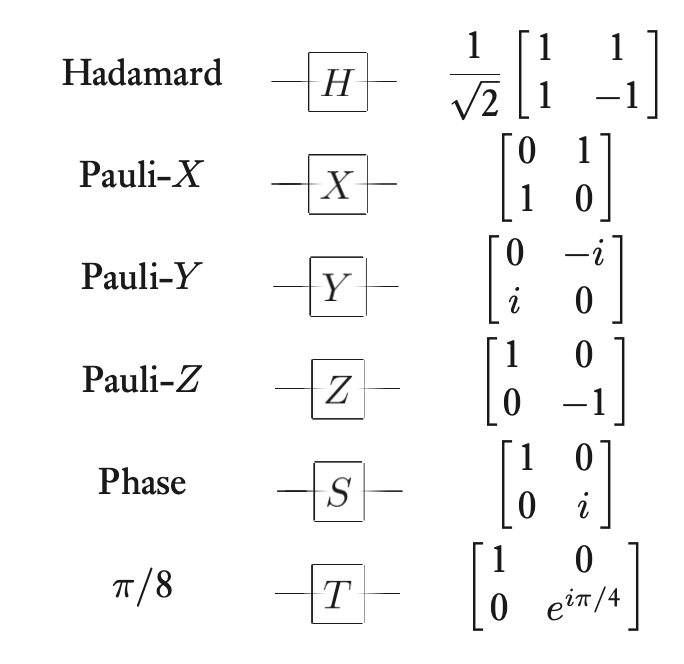
\includegraphics[width=0.5\linewidth]{images/qubit_gates.png}
    \caption{Qubit Gates \autocite[177]{nielsen_quantum_2010}}
    \label{fig:enter-label}
\end{figure}

\begin{itemize}
    \item Das Hadamard-Gate (H) bringt Qubits aus Ihren Basiszuständen in eine Superposition 
    \item Das CNOT-Gate (Controlled-Not), ist ein zwei Qubit Gate, welches als zentraler Bestandteil der Quantenverschränkung funktiert, es verschränkt sozusagen zwei Qubits miteinander 
    \item Neben diesen beiden sehr wichtigen Gates gibt es auch noch die Pauli-X, -Y. und -Z Gates, sowie Phasengatter, T-Gate  und weitere 
\end{itemize}
Werden mehrerer dieser Gatter nacheinander auf ein Qubit Register angewendet, bildet sich daraus ein Quanten-Schaltkries, welcher als gesamter Algorithmus verstanden werden kann.
\autocite[174-188]{nielsen_quantum_2010}
\subsection*{Bekannte Quantenalgorithmen basierend auf dem Quantenschaltkreismodell}
Das Quantenschaltkreismodell dient als Grundlage für mehrere bekannte Quantenalgorithmen dazu zählen folgende: (siehe auch (\autoref{basic_algorithms}))
\subsubsection*{1) Shor's Algorithmus}
Der Shor Algorithmus führt eine effiziente Primfaktorzerlegung großer Zahlen durch, was klassische Verschlüsselungsverfahren wie RSA bedroht. Der Algorithmus verwendet die Quantum Fourier Transformation (QFT) und periodenfindende Subroutinen innerhalb des Circuit-Models. (siehe auch (\autoref{first:shor-algorithm}) \autocite[226-232]{nielsen_quantum_2010} \textbf{hier fehlt noch die Quelle "Quantum Computing  and Shor´s Algorithmus"}
\subsubsection*{2) Grover´s Algorithmus}
Der Grover Algorithmus dient zur Suche eines Eintrags in einer unstrukturierten Datenbank mit einer quadratischen Beschleunigung gegenüber klassischen Verfahren.
Der Algorithmus basiert auf Rotation in einem zweidimensionalen Unterraum, dargestellt als wiederholte Anwendung von sogenannten Grover-Iterationen, realisiert durch Gates im Circuit-Modell. (ausführliche Erklärung: (\autoref{sec:grover-algorithm}))  \autocite[248-254]{nielsen_quantum_2010}

\subsubsection*{3) Regev}
Regevs Arbeiten zum LWE-Problem beinhalten eine theoretische Quantenreduktion, die sich vollständig im gate-basierten Modell realisieren lässt. Die dafür erforderlichen Operationen – wie das Erzeugen von Superpositionen, die Anwendung der Quanten-Fouriertransformation sowie die Verarbeitung von Messresultaten – sind mit klassischen Quanten-Gattern (z.B. Hadamard-, CNOT- und Phasengattern) darstellbar. Auch wenn Regevs Reduktion primär theoretischer Natur ist und keine praktischen Implementierungen wie Shor oder Grover hat, zeigen die verwendeten Techniken eine klare Kompatibilität mit dem Quantum Circuit Model. \autocite{regev_lattices_2024}


Das gate-basierte Paradigma ist nicht nur ein theoretisches Modell, das man in der Quanteninformatik zur Beschreibung von Algorithmen verwendet – es spielt auch in der Praxis eine zentrale Rolle. So setzt zum Beispiel das Open-Source-Framework Qiskit von IBM genau auf dieses Modell: Quantenprogramme werden dort direkt als sogenannte „Quantum Circuits“ aufgebaut. Diese bestehen aus einer festen Anzahl von Qubits und einer Folge von Operationen, also Gattern, Messungen und Resets – genau wie es im Schaltkreis-Modell vorgesehen ist.
Dass Theorie und Praxis hier so eng zusammenhängen, zeigt, wie wichtig das gate-basierte Modell nicht nur für die Entwicklung von Algorithmen ist, sondern auch für den praktischen Einsatz auf echten Quantencomputern, wie denen von IBM oder Google.

\subsection{Messungsbasiertes Paradigma}
Das messungsbasierte Paradigma, auch bekannt als Measurement-Based Quantum Computing (MBQC) oder one-way quantum computation, stellt eine alternative Architektur zur Implementierung von Quantenalgorithmen dar. Im Gegensatz zum weit verbreiteten Schaltkreis-Modell, bei dem Quanteninformationen durch sequenzielle Anwendung unitärer Gatter verarbeitet werden, basiert MBQC auf einer anderen Grundidee: Der eigentliche Rechenprozess erfolgt nicht durch Gatter, sondern ausschließlich durch gezielte Einzelqubit-Messungen an einem vorbereiteten, verschränkten Vielteilchenzustand – dem sogenannten Cluster-State.
Diese Struktur eröffnet neue Perspektiven auf die Organisation und Steuerung von Quanteninformation. Die gesamte logische Verarbeitung geschieht dabei einseitig – also „one-way“ – da jede Messung irreversibel ist und den gemessenen Qubit-Zustand zerstört. Die Fähigkeit zur universellen Quantenberechnung wird dabei vollständig durch die Verschränkungseigenschaften des vorbereiteten Zustands sowie die geschickte Wahl und Abfolge der Messungen realisiert. \autocite[2-4]{briegel_measurement-based_2009}
\subsection*{Struktur und Erzeugung von Cluster-States}
Zentrale Ressource des MBQC ist der Cluster-State, ein hochgradig verschränkter Quantenzustand mehrerer Qubits. Formal gehört der Cluster-State zur Klasse der Graphenzustände. Diese Zustände lassen sich durch mathematische Graphen beschreiben, in denen Knoten einzelnen Qubits entsprechen und Kanten die Verschränkungen zwischen ihnen darstellen.

Die Erzeugung eines solchen Zustands erfolgt in zwei Schritten:
\begin{enumerate}
    \item 	Zunächst werden alle Qubits in den Zustand $|+\rangle = \frac{1}{\sqrt{2}}(|0\rangle + |1\rangle)$ gebracht.
    \item 2.	Anschließend wird auf jedes benachbarte Qubitpaar (gemäß der Graphstruktur) ein kontrolliertes Phasengatter $U_{PG}=diag(1,1,1,-1)$ angewendet.
\end{enumerate}
Der so erzeugte Zustand $|G\rangle$, wobei G der zugrundeliegende Graph ist, besitzt die gewünschten Verschränkungseigenschaften, um ihn als Rechenressource im MBQC zu verwenden. Besonders der zweidimensionale (2D) Cluster-State hat sich hierbei als universell erwiesen, d.h. als hinreichend mächtig für die Implementierung beliebiger Quantenalgorithmen (vgl. \textbf{FIX REF} ebenda \citeyear{h_j_briegel_measurement-based_2009}, S. 2-3).
\subsection*{Rechenmodell und Algorithmus Implementierung}
Eine MBQC-Berechnung lässt sich in einem schematischen Ablauf darstellen, der vier grundlegende Schritte umfasst:
\begin{enumerate}
    \item \textbf{Initialisierung:} Vorbereitung eines ausreichend großen 2D-Cluster-States, der unabhängig vom konkreten Algorithmus erzeugt wird.
    \item \textbf{Kodierung des Algorithmus durch Messmuster:} Die Berechnung wird durch eine Sequenz von Einzelqubit-Messungen in ausgewählten Basen realisiert. Dabei bestimmt das Muster der Messungen (also deren Reihenfolge und jeweilige Basis) die Art der durchgeführten logischen Operationen.
    \item \textbf{Adaptive Steuerung:} Die Wahl der Messbasis für spätere Schritte kann von den Ergebnissen vorheriger Messungen abhängen. Diese Feedforward-Kontrolle wird durch eine klassische Recheneinheit übernommen.
    \item \textbf{Ausgabezustand:} Das Endresultat der Quantenberechnung ist entweder in den verbleibenden nicht gemessenen Qubits codiert oder ergibt sich aus den Messergebnissen selbst. Die resultierenden Zustände unterscheiden sich höchstens durch lokale Pauli-Operationen.
\end{enumerate}
Ein bemerkenswertes Merkmal dieses Modells ist, dass trotz der inhärenten Zufälligkeit der einzelnen Messergebnisse (aufgrund des quantenmechanischen Messprozesses) der gesamte Rechenvorgang deterministisch kontrolliert und wiederholbar bleibt – vorausgesetzt, das Feedforward wird korrekt berücksichtigt (vgl. \textbf{FIX REF} ebenda \citeyear{h_j_briegel_measurement-based_2009}, S. 3-4).
\subsection*{Exemplarische Anwendungen}
Das Potential des MBQC lässt sich gut an ausgewählten Beispielen verdeutlichen. Eines der grundlegendsten Konzepte ist das Teleportationsprotokoll, das im Kontext des MBQC zeigt, wie Quanteninformation durch Messungen effektiv von einem Teil des Clusters zum anderen übertragen werden kann. Dieses Prinzip bildet die Basis für viele weiterführende Techniken, darunter auch die Realisierung effektiver logischer Gatter allein durch Messungen.
Darüber hinaus lassen sich bekannte Algorithmen wie der Shor-Algorithmus zur Faktorisierung großer Zahlen oder der Grover-Algorithmus zur Datenbanksuche in messungsbasierten Varianten formulieren. Diese benötigen lediglich eine geeignete Struktur des zugrunde liegenden Cluster-States sowie eine korrekt gewählte Messstrategie, um dieselbe Funktionalität wie im Schaltkreis-Modell zu erreichen. Damit zeigt sich die formale Äquivalenz der beiden Paradigmen – bei grundlegend unterschiedlicher Umsetzung (vgl. \textbf{FIX REF} ebenda \citeyear{h_j_briegel_measurement-based_2009}, S. 2)

\subsection{Adiabatisches Paradigma (Quantum Annealing)}
Ein weiteres Modell zur Realisierung von Quantenalgorithmen ist das adiabatische Paradigma, welches auch als "Quantum Annealing" bezeichnet wird. Das Adiabatischen Modell basiert auf der Idee, ein Quantensystem durch eine langsame, kontinuierliche Änderung eines Hamiltonians gezielt in seinen Grundzustand zu führen. Die gesuchte Lösung des Modells ist in diesem Grundzustand markiert. Genau in dieser Art unterscheidet sich das Quantum Annealing auch vom Gate oder messungsbasierten Modell. 
Das Grundprinzip des Modells besteht darin, dass man das Quantensystem zunächst in einem leicht vorbereiteten Anfangszustand hält. Dieser entspricht dem Grundzustand eines sogenannten Treibenden Hamiltonians $H_D$. Dieser Hamiltonian kann z.B. ein transversales Feld enthalten, das alle Qubits gleichmäßig beeinflusst. Im Laufe des Algorithmus wird dann schrittweise der Problem-Hamiltonian $H_P$ zugeschaltet, dieser enthält die Struktur des zu lösenden Problems. Die Gesamtentwicklung erfolgt über einen zeitabgängigen Hamiltonian, der folgenden Form:
$$
H(t) = A(t) \cdot H_D + B(t) \cdot H_P
$$

Die beiden Funktionen A(t) und B(t) steuern, wie stark der jeweilige Hamiltonian zu einem bestimmten Zeitpunkt t wirkt. Am Anfang dominiert hierbei $H_D$ und am Ende $H_P$. Das System bleibt nach dem adiabatischen Theorem während des gesamten Prozesses im jeweiligen Grundzustand, wenn die Änderungen langsam genug erfolgen. Am Ende wird die gesuchte Lösung, also der Grundzustand von $H_P$ erreicht.
 
Die Hamiltonian dürfen mit einer Geschwindigkeit geändert werden, die stark vom sogenannten Energieabstand (Gap) zwischen dem Grundzustand und dem ersten angeregten Zustand abhängt. Je kleiner dieser Abstand ist, desto langsamer muss die Änderung erfolgen, um unerwünschte Übergänge in angeregte Zustände zu vermeiden. 
Das Quantum Annealing eignet sich besonders gut für kombinatorische Optimierungsprobleme, da viele davon auf sogenannte Ising-Modelle abgebildet werden können. Ein Beispiel für ein Problem-Hamiltonian ist folgendes:
$$
H_P = \sum_{i,j} J_{ij}\sigma_i^z\sigma_j^z + \sum_i h_i\sigma_i^z
$$
Die Kopplungsterme $J_{ij}$ und die lokalen Felder $h_i$ kodieren hierbei die jeweilige Problemstruktur.
Es gibt verschiedene Problemklassen, welche durch Quantum Annealing gelöst werden können, zu den typischen gehören unter anderem Folgende Beispiele: 
\begin{itemize}
    \item \textbf{Max-Cut: }Bei Max-Cut wird ein Graph aufgeteilt in zwei Teilmengen, sodass die Kantensumme zwischen den beiden Mengen maximal wird 
    \item 	\textbf{k-Clique:} Bei der k-Clique-Suche geht es darum, vollständige Teilgraphen mit genau k Knoten zu finden, also Untergruppen, in denen jeder Knoten mit jedem anderen verbunden ist 
    \item \textbf{Graph Coloring: }Beim Graph Coloring sollen Knoten eines Graphen mit möglichst wenigen Farben so eingefärbt werden, dass benachbarte Knoten unterschiedliche Farben erhalten 
    \item \textbf{Ising-Modell-Minimierung:} Hier wird der Ising-Hamiltonian direkt minimiert. Da sich viele kombinatorische Probleme darauf abbilden lassen, bildet diese Minimierung die Grundlage für zahlreiche Optimierungsaufgaben 
\end{itemize}
Quantum Annealing (QA) verwendet im Gegensatz zum klassischen Simulated Annealing (SA), bei der thermische Fluktuationen benutzt werden, Quantenfluktuationen, insbesondere Quanten-Tunnel, um Energiebarrieren zu überwinden. Das ist vor allem dann ein Vorteil, wenn die Energiebarrieren hoch, aber schmal sind. In genau diesen Fällen kann das Quantum Annealing schneller zu einer optimalen Lösung finden als sein klassischen Gegenstück Simulated Annealing. 
Das adiabatische Paradigma wurde in der Praxis unter anderem durch die Firma D-Wave Systems in Hardware umgesetzt. Die Systeme von D-Wave Systems sind darauf spezialisiert Optimierungsprobleme durch Quantum Annealing zu lösen, also das adiabatische Paradigma technisch zu realisieren. \autocite[2-4]{rajak_quantum_nodate} \autocite[4-5, 42-43]{albash_adiabatic_2018}
\subsection{Hybrid-Paradigma}
Das Hybrid-Paradigma stellt neben dem Gate basierten und adiabatischen Modell einen weiteren wichtigen Ansatz zur Realisierung von Quantenalgorithmen dar. Es ist aus dem Grund besonders interessant, da es sowohl klassische als auch quantenmechanische Bestandteile kombiniert. Konkret bedeutet das, dass die aufwendigen und hardwareintensiven Berechnungen, wie etwa die Manipulation und Messung von Quantenzuständen auf dem Quantencomputer laufen, während Aufgaben wie das Anpassen von Parametern oder das Auswerten von Messergebnissen klassisch bearbeitet werden. Aufgrund dieser Aufgabenteilung lassen sich viele Probleme bereits heutzutage auf existierender Hardware lösen. Das liegt vor allem daran, dass das Hybrid-Paradigma mit relativ kurzen Quantenschaltungen auskommt und keine langen kohärenten Entwicklungen benötigt. \autocite[1-2]{cerezo_variational_nodate}
Das Grundprinzip im Hybrid-Paradigma ist immer gleich. Man startet zunächst mit einem Anfangszustand, der mithilfe einer parametrierten Quantenschaltung erzeugt wird. Anschließend wird ein Zielwert gemessen, das kann z.B. eine Energie sein und gibt dann diesen Messwert an den klassischen Computer zurück. Auf diesem wird dann ein Optimierungsalgorithmus ausgeführt, der neue Parameter vorschlägt, mit denen die Quantenschaltung beim nächsten Durchlauf verändert wird. Dieser Prozess wird so lange wiederholt, bis ein gewünschtes Ergebnis erreicht ist. Das erklärte Prinzip kommt in mehreren hybriden Algorithmen zum Einsatz. Im Folgenden werden nun drei bekannte hybride Algorithmen genauer vorgestellt. 
\subsubsection*{1) Variationaler Quanten Eigenlöser (VQE)}
Der variationale Quanten Eigenlöser (engl, variational quantum eigensolver), kurz VQE, ist ein hybrider Algorithmus der Berechnung von Eigenwerten, genauer gesagt zur Bestimmung des Grundzustands eines Hamiltonians verwendet wird. In der Quantenchemie ist das extrem wichtig, da sich damit die Energie eines Moleküls berechnen lässt. Die Idee hinter dem VQE-Algorithmus ist es einen Quantenzustand $|\psi(\theta)\rangle$ vorzubereiten, der von bestimmten Parametern $\theta$ abhängt. Für diesen Zustand wird dann der Erwartungswert einer Energie gemessen, was sich mathematisch durch folgende Formel ausdrücken lässt:
$$
\langle\psi(\theta)|H|\psi(\theta)\rangle
$$
Dieser Ausdruck wird als sogenannte Kostenfunktion verwendet. Das Ziel ist es die Parameter θ so zu verändern, dass die gemessene Energie möglichst klein wird und somit dem Grundzustand des Systems entspricht. Dieser Schritt passiert auf einem klassischen Rechner, der z.B. den Nelder-Mead-Algorithmus oder einen anderen Optimierer nutzt, nicht auf dem Quantencomputer selbst. 
Ein großer Vorteil von VQE ist, dass die benötigten Quantenschaltungen relativ flach bleiben, sie kommen mit wenigen Gattern und kurzen Operationen aus. Diese Tatsache ist besonders für NISQ-Hardware praktisch, da bei dieser jede zusätzliche Operation das Risiko für Fehler erhöht. \label{nisq-definition}
2014 wurde der VQU bereits durch Peruzzo et al, erfolgreich auf einem photonischen Quantenprozessor umgesetzt. Dabei wurde die Bildungskurve des Moleküls He–H⁺ berechnet. Die Energie wurde dabei über ein klassisch-quantisches Zusammenspiel optimiert und das Ergebnis lag innerhalb der chemischen Genauigkeit. Das war bereits ein starker Beweis dafür, dass hybride Algorithmen schon vor über 10 Jahren auf damaliger Hardware praktikabel waren. 
(vgl. \citeauthor{cerezo_variational_nodate}, \citeyear{cerezo_variational_nodate}, vgl. \citeauthor{peruzzo_variational_nodate}, \citeyear{peruzzo_variational_nodate})
\subsubsection*{2) Quantum Approximate Optimization Algorithm (QAOA)}
Der sogenannte Quantum Approximate Optimization Algorithm (QAOA) ist ein weiterer Algorithmus des Hybrid-Paradigmas und wurde dazu entwickelt, um kombinatorische Optimierungsprobleme zu lösen. Typische Beispiele hierfür sind Max-Cut, k-Clique oder andere Graph Probleme (siehe Kapitel…). Auch QAOA besteht aus einem parametrisierten Quantenschaltkreis und einer klassischen Optimierung, funktioniert jedoch deutlich anders als VQE.
Das Verfahren nutzt zwei Hamiltonians. Einmal einen Probleme-Hamiltonian $H_C$, welcher das zu lösende Problem abbildet (z.B. ein Ising-Modell) und einmal einen sogenannten Mixer-Hamiltonian $H_B$, der typischerweise eine Summe von X-Gattern ist. Ausgehend vom Anfangszustand werden nun abwechselt die Hamiltonian $H_C$ und $H_B$ auf das System angewendet. Daraus ergibt sich dann für eine Schaltungstiefe p folgender QAOA-Zustand: 
$$
|\psi_p(\vec{\gamma}, \vec{\beta})\rangle = e^{-i\beta_p H_B}e^{-i\gamma_p H_C} \dots e^{-i\beta_1 H_B}e^{-i\gamma_1 H_C} |+\rangle^{\otimes N}
$$
(vgl. \citeauthor{zhou_quantum_nodate}, \citeyear{zhou_quantum_nodate}, S. 3 Gleichung (3))


Die Parameter $\gamma$ und $\beta$ werden dabei von einem klassischen Optimierer so angepasst, dass die gemessene Erwartung des Zieloperators optimiert wird. Das System bleibt hierbei anders als beim adiabatischen Paradigma nicht unbedingt im Grundzustand, sondern nutzt gezielt nicht-adiabatische Übergänge, um effizient zu besseren Lösungen zu kommen. Damit eignet sich der Algorithmus gut für NISQ-Geräte und kann mit relativ flachen Quantenschaltungen implementiert werden. 
(vgl. \citeauthor{zhou_quantum_nodate}, \citeyear{zhou_quantum_nodate}, S. 2-9)

\subsubsection*{3) Quantum Machine Learning}
Das letzte der drei genannten typischen Gebiete in dem hybride Quantenalgorithmen eine wichtige Rolle spielen, ist das sogenannte Quantum Machine Learning. Hierbei kommt es wie der Name schon vermuten lässt zur Verbindung von Quantencomputing und maschinellem Lernen. Auch in diesem Gebiet ist das Hybrid-Paradigma der Standard, weil klassische Daten verarbeitet und mit quantenmechanischen Methoden analysiert werden. 
Hierbei läuft das typische Vorgehen wie folgt ab. Zunächst werden die Eingangsdaten, also z.B. Bilder oder numerische Werte, durch sogenannte Feature Maps in einen Quantenzustand umgewandelt. Anschließend wird dieser Zustand durch eine parametrisierte Quantenschaltung geschickt die als Klassifikator dient. Abschließend wird das Ergebnis auf einem klassischen Computer ausgewertet und der Fehler wird klassisch minimiert. 
Ein Beispiel für Quantum Machine Learning ist der Variational Quantum Classifier (VQC), bei dem die Quantenschaltung so trainiert wird, dass sie zum Beispiel zwischen verschiedenen Klassen unterscheiden kann, wie z.B. zwischen verschiedenen Ziffern in einem Bild. Auch hier wird eine Kostenfunktion (z.B. der Klassifikationsfehler) iterativ durch einen klassischen Optimierer minimiert. 
Ein großer Vorteil und damit eine Stärke des hybrides Ansatzes von Quantum Machine Learning liegt darin, dass man quantenmechanische Effekte wie die Superposition und Verschränkung nutzen kann, um komplexe Strukturen in Daten zu erkennen und dabei aufgrund des Machine Learning nicht auf eine vollständige Quantenhardware angewiesen ist.

(vgl. \citeauthor{alchieri_introduction_2021}, \citeyear{alchieri_introduction_2021}, S.2-4)


Das Hybrid-Paradigma ist ein zentraler Baustein moderner Quantenalgorithmen. Es ist besonders gut für aktuelle NISQ-Geräte geeignet und ermöglicht die Zusammenarbeit zwischen klassischem Rechner und Quantenprozessor. Hybride Verfahren zeigen bereits heute, egal ob in der Quantenchemie, bei Optimierungsproblemen oder in maschinellem Lernen, was auf echter Hardware möglich ist. Sie gelten als vielversprechender Weg in Richtung praktischer Quantenanwendungen. 

\subsection{Funktionelles Paradigma}

\setlength{\parindent}{0pt} % Keine Einrückung am Absatzanfang
\setlength{\parskip}{1em}   % Fügt einen vertikalen Abstand von 1em zwischen Absätzen ein

Das funktionelle Paradigma im Quantencomputing verfolgt den Ansatz, Quantenprogramme als Funktionen zu modellieren, vergleichbar mit klassischen funktionalen Programmiersprachen. Es ermöglicht eine deklarative, abstrahierte und zugleich formal fundierte Beschreibung quantenmechanischer Prozesse und hebt sich damit deutlich von den herkömmlichen, zumeist schaltkreisorientierten Programmiersprachen ab. Ein zentrales Beispiel ist die Sprache QML (Quantum Meta Language), in der Programme als Ausdrücke formuliert werden, deren Bedeutung sich durch morphische Abbildungen innerhalb der Kategorie endlicher Quantenberechnungen (FQC) erschließt. Diese formale Semantik erlaubt es, sowohl reversible als auch irreversible Quantenoperationen in einer gemeinsamen Sprache zu erfassen.

Ein wesentliches Anliegen dieses Paradigmas ist die gezielte Kontrolle von Dekohärenz -- einem der kritischsten Probleme in der praktischen Umsetzung von Quantenalgorithmen. QML begegnet dieser Herausforderung mit einem strikt linearen Typ-System, das sicherstellt, dass jede Variable, insbesondere jeder Qubit, genau einmal verwendet wird. Dadurch wird die Einhaltung quantenmechanischer Prinzipien wie des No-Cloning-Theorems gewährleistet. Operationen, die eine Messung des Zustands erzwingen, wie etwa \texttt{if}, werden dabei syntaktisch von solchen unterschieden, die ohne Dekohärenz auskommen, wie \texttt{if\textsubscript{$\circ$}}. Letztere dürfen nur unter orthogonalitätsbasierten Bedingungen verwendet werden, was eine formale Absicherung gegen unbeabsichtigte Messprozesse bietet. Auf diese Weise lassen sich Superpositionen und Verschränkungen programmatisch erhalten und präzise steuern.

Die Ausdrucksstärke des funktionellen Paradigmas zeigt sich besonders in der formalen Darstellung bekannter Quantenalgorithmen und -protokolle. Grundlegende Operationen wie das Hadamard-Gatter oder Variationen von Deutsch's Algorithmus lassen sich in QML nicht nur elegant formulieren, sondern auch direkt in Quanten-Schaltkreise überführen. Die Algorithmen von Shor und Grover, auf die in den Abschnitten \ref{sec:Shor-Algorithmus} und \ref{sec:grover-algorithm} eingegangen wird, können ebenfalls in diesem Rahmen abgebildet werden. Darüber hinaus eignet sich QML hervorragend zur Beschreibung komplexer Quantenprotokolle wie etwa Superdense Coding. Die Sprache erlaubt es, parallele Auswertungen mehrerer Qubits strukturell auszudrücken, was die zugrunde liegenden Prinzipien des Quantenparallelismus nicht nur sichtbar macht, sondern auch formal überprüfbar werden lässt.

Eine der größten Stärken des funktionellen Paradigmas liegt schließlich in der Transparenz des Ressourcenmanagements. Da Weakenings -- also das bewusste Ignorieren oder Nicht-Nutzen von Variablen -- explizit gekennzeichnet werden müssen, lassen sich die Stellen im Programm eindeutig identifizieren, an denen Dekohärenz eintritt. Dies eröffnet die Möglichkeit einer gezielten Optimierung hinsichtlich der Informationssicherheit und der quantenmechanischen Integrität eines Programms.

Insgesamt stellt das funktionelle Paradigma eine leistungsfähige und theoretisch fundierte Grundlage für die Entwicklung und Verifikation von Quantenprogrammen dar. Es verbindet formale Strenge mit praktischer Anwendbarkeit und erlaubt es, sowohl algorithmische als auch protokollbasierte Quantenoperationen in einem klar typisierten, kontrollierten und analysierbaren Rahmen zu formulieren (vgl. \citeauthor{thorsten_altenkirch_functional_2005}, \citeyear{thorsten_altenkirch_functional_2005}).


\section{Quanten-Programmiersprachen und -Frameworks}
\label{sec:programming-languages}

Die Entwicklung von Quantencomputern hat zur Entstehung spezialisierter Programmiersprachen und Frameworks geführt, die die besonderen Eigenschaften des Quantencomputings berücksichtigen. Diese Sprachen und Frameworks ermöglichen es Entwicklern, Quantenalgorithmen zu implementieren und zu testen, ohne sich mit den komplexen physikalischen Details der Quantenhardware auseinandersetzen zu müssen.

Im Gegensatz zu klassischen Programmiersprachen müssen Quanten-Programmier-sprachen spezielle Konzepte wie Superposition, Verschränkung und Messung unterstützen. Sie müssen auch die Interaktion zwischen klassischen Berechnungen und Quantenberechnungen ermöglichen, da die meisten Quantenalgorithmen sowohl klassische als auch Quantenkomponenten enthalten.

Dieses Kapitel gibt einen Überblick über die verschiedenen Arten von Quanten-Programmiersprachen und ordnet sie den vorangegangenen Programmierparadigmen zu. Anschließend wird das Framework Qiskit von IBM detaillierter betrachtet.

\subsection{Übersicht über Sprachen und Frameworks}
Quanten-Programmiersprachen lassen sich nach unterschiedlichen Dimensionen systematisch klassifizieren. Diese betreffen die Abstraktionsebene, das Programmierparadigma, die Hardwarebindung sowie das zugrundeliegende Quantenmodell. Eine klare Trennung dieser Dimensionen erleichtert die Einordnung und den Vergleich der verschiedenen Ansätze. In diesem Kapitel werden diese zentrale Unterscheidungsmerkmale systematisch dargestellt. Zu jeder Kategorie werden exemplarische Sprachen vorgestellt, welche abschließend in einer vergleichenden Übersichtstabelle gegenübergestellt werden.

\textbf{Abstraktionsebenen}\\ 
Die Abstraktionsebene einer Quantenprogrammiersprache oder eines entsprechenden Frameworks definiert den Grad der Nähe des Codes zur physikalischen Quantenhardware beziehungsweise die Höhe der konzeptionellen Abstraktionsebene, auf der die Programmierung erfolgt.
Man unterscheidet zwischen High-Level- und Low-Level-Sprachen. 

\textit{Low-Level-Sprachen} ermöglichen die Kontrolle über einzelne Qubits und Quantengatter. Sie orientieren sich stärker an konkreten Schaltkreisen und hardware-nahen Operationen. Ein Beispiel hierfür ist OpenQASM, das als Assemblersprache für Quantencomputer dient. Es ermöglicht eine präzise Steuerung der Quantenschaltkreise, erfordert jedoch auch ein tiefes Verständnis der Quantenmechanik und Hardware-Architektur (Vgl. \cite{cross_open_2017}).

\textit{High-Level-Sprachen} hingegen bieten eine größere Abstraktion, die es Entwicklern ermöglicht, sich auf die Logik des Quantenalgorithmus zu konzentrieren und Algorithmen unabhängig von konkreten Schaltkreisen zu beschreiben. Sie ähneln klassischen Programmiersprachen und sind intuitiver zu bedienen, indem sie die Komplexität von Quantenoperationen abstrahieren. Beispiele hierfür sind Q\#, Qiskit oder Cirq, die im späteren Verlauf dieses Kapitels genauer betrachtet werden (Vgl. \cite{singh_survey_2024})

\textbf{Programmierparadigmen}\\ 
Das Programmierparadigma beschreibt den stilistischen und konzeptionellen Ansatz der Formulierung und Organisation von Programmen.

\textit{Imperative Programmiersprachen}, auch prozedurale Sprachen genannt, sind im Quantum-Computing von klassischen imperativen Sprachen wie C oder Java inspiriert und verwenden meist das QRAM-Modell. Sie basieren auf Anweisungen, die den globalen Zustand eines Programms ändern (Vgl. \cite{garhwal_quantum_2021}). 

Das Quanten-Schaltkreismodell gilt als treibende Kraft der Quantenprogrammierung. Um dieses in eine Sprache einzubauen, wurde ein Pseudocode für die Quantenprogrammierung vorgeschlagen, der in der Sprache QCL mündete. Als erste imperative Quantum-Programmiersprache wurde sie im Jahr 1998 an der technischen Universität in Wien veröffentlicht. QCL verwendet hierbei eine von C abgeleitete Syntax und bietet einen vollständigen Quantensimulator für die Codeentwicklung auf einem klassischen Computer (Vgl. \cite{sofge_survey_2008}).

Quantum Guarded Command Language (qGCL) als weitere imperative Sprache basiert auf Dijkstras Semantik der Programmiersprache und hat verschiedene Konzepte wie das Quantenregister in Form eines Vektors eingeführt. LanQ ist eine high-level, imperative Quantenprogrammiersprache, deren Syntax ebenfalls der Sprache C ähnelt. Sie führt Quantenberechnungen unter Verwendung der klassischen Steuerung auf Quantendaten durch. LanQ wurde entwickelt, da QCL und qGCL keine Interprozesskommunikation und Mehrparteienprotokolle unterstützen. Bei LanQ gehört jede Quantenressource höchstens einem Prozess an, während der Kanal von Sender- und Empfängerprozess gemeinsam genutzt werden kann. Darüber hinaus bietet LanQ Werkzeuge für die parallele Ausführung von Programmen (Vgl. \cite{garhwal_quantum_2021}).

In \textit{funktionalen, deklarativen Sprachen} werden Berechnungen mit Hilfe mathematischer Funktionen durchgeführt, die auf Konzepte wie dem Lambda-Kalkül und der linearen Logik zurückgreifen. Lambda-Kalküle sind Konstruktionen aus der mathematischen Logik und können als die kleinsten universellen Programmiersprachen betrachtet werden. Sie bestehen aus einer einzigen Transformationsregel (Variablensubstitution) und einem einzigen Funktionsschema. Jede berechenbare Funktion kann mit diesem Formalismus ausgedrückt werden (Vgl. \cite{garhwal_quantum_2021}).

Quantum ML (QML) ist eine funktionale Quantensprache aus dem Jahr 2006. QML Programme sind frei von Dekohärenz und gewährleisten Quantenparallelität durch Superposition und Verschränkung (Vgl. \cite{garhwal_quantum_2021}). 
Quipper ist eine weitere high-level, skalierbare und funktionale Quantenprogrammiersprache. Sie wurde zur Programmierung einer Reihe von nicht-trivialen Quantenalgorithmen verwendet und kann Darstellungen mit Billionen von Gattern erzeugen. Quipper ist auf ein Berechnungsmodell ausgerichtet, das einen klassischen Computer zur Steuerung eines Quantengeräts verwendet und ist dabei nicht von einer bestimmten Quantenhardware abhängig (Vgl. \cite{green_quipper_2013}). Eine vergleichbare klassische Programmiersprache ist Haskell.

\textit{Hybride, multi-Paradigmen Sprachen} und Frameworks kombinieren imperative Programmierung und deklarative Schaltungen. Sie integrieren sowohl klassische als auch Quantenprogrammierkonzepte, um komplexe Interaktionen zwischen verschiedenen Algorithmen zu ermöglichen und beide Berechnungsarten zu kombinieren. Dies ist in der heutigen NISQ-Ära von hoher Relevanz. Diese Ära beschreibt den aktuellen technologischen Übergangszeitraum der Quanteninformatik, in der erste Quantenalgorithmen zwar auf realen Geräten ausführbar, aber noch fehlerhaft, klein und begrenzt sind (Vgl. \ref{nisq-definition}). 

Eine hybride, domänenspezifische Quantenprogrammiersprache ist Q\# als Teil des Microsoft Quantum Development Kits. Sie besteht aus einem kleinen Satz von primitiven Datentypen, Arrays und Tupeln zur Erstellung neuer strukturierter Datentypen und unterstützt if-then Anweisungen und Schleifen. Weitere Merkmale umfassen die Interoperabilität mit der Python-Programmierung sowie die Unterstützung des Verschränkungs- und Überlagerungskonzepts (Vgl. \cite{garhwal_quantum_2021}).

In Abbildung \ref{fig:quantum-landscape} ist eine Übersicht über diverse Programmiersprachen nach Abstraktionsebene und Programmierparadigmen (Type of language) zu sehen. Die Abbildung verdeutlich jedoch auch, dass es bislang keine einheitlich standardisierte Klassifikation von Quantenprogrammiersprachen gibt und diese je nach Quellen variiert. Während \citeauthor{garhwal_quantum_2021} Q\# als eine hybride Programmiersprache hervorgehoben haben, ordnen \citeauthor{serrano_quantum_2023} sie dem imperativen Paradigma zu. Unterschiedliche Autoren setzen dabei teils unterschiedliche Schwerpunkte, was zu divergierenden Einordnungen führen kann. Angesichts der uneinheitlichen Einordnungen in der Literatur erscheint die Erarbeitung eines standardisierten Klassifikationsschemas als eine relevante Aufgabe für zukünftige Forschungsarbeiten.

\begin{figure}[H]
    \centering
    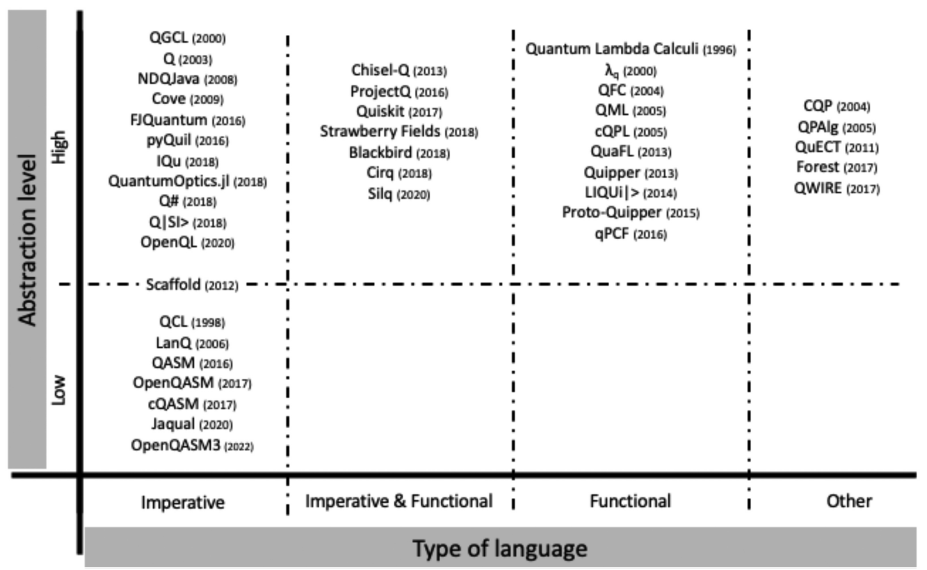
\includegraphics[width=0.9\linewidth]{images/languages/Quantum-Programming-Landscape.png}
    \caption{Übersicht über Quanten-Programmiersprachen nach Abstraktionsebenen und Programmierparadigmen (\cite{serrano_quantum_2023})}
    \label{fig:quantum-landscape}
\end{figure}

\textbf{Hardwarebindung}\\
Die Hardwarebindung einer Quanten-Programmiersprache oder eines Frameworks beschreibt, inwieweit sie an eine bestimmte Quantenhardware-Plattform gebunden ist. Man unterscheidet zwischen Hardware-spezifisch und Hardware-unabhängig.

\textit{Hardware-Spezifische} Frameworks sind für die Optimierung und Ausführung auf einer bestimmten Architektur konzipiert und optimiert. Sie nutzen die spezifischen Eigenschaften und Einschränkungen der Hardware zur Maximierung der Leistung. Beispiele hierfür sind Cirq, optimiert für Google Sycamore Hardware (https://quantumai.google/cirq) oder PyQuil, optimiert für Rigetti´s Quantum Cloud Service. (https://www.rigetti.com/what-we-build). #INTERNETQUELLEN NOCH ANPASSEN

\textit{Hardware-unabhängige}Sprachen und Frameworks sind so konzipiert, dass sie auf einer Vielzahl von Hardware-Plattformen ausgeführt werden können, oft durch die Verwendung von Zwischenrepräsentationen wie OpenQASM. Sie bieten eine große Flexibilität und Portabilität. Zu ihnen gehören unter anderem Qiskit von IBM sowie Q\# von Microsoft.

\textbf{Quantenmodell}\\ 
Eine weitere wesentliche Klassifikationsdimension ergibt sich aus dem zugrunde liegenden Quantenmodell. Quantencomputer können auf verschiedenen physikalischen Prinzipien und Berechnungsmodellen basieren, die sich auch in den Programmiersprachen widerspiegeln. Hierfür werden Programmiersprachen den Modellen aus \ref{programming-models} zugeordnet.

Das Gate-basierte Modell ist das dominanteste und am weitesten verbreitete Modell, bei dem Quantenalgorithmen durch Schaltkreise aus Quantengattern auf Qubits dargestellt werden. Ein Großteil der aktuellen Quantencomputer und Frameworks basieren auf diesem Modell. Beispiele für Sprachen und Frameworks sind die bereits erwähnten Qiskit, Cirq oder OpenQASM (Vgl. \cite{QUELLE FEHLT})

Das messungsbasierte Paradigma (MBQC) führt Berechnungen durch eine Sequenz von Einzel-Qubit-Messungen auf einem vorbereiteten hochgradig verschränkten Anfangs-Cluster-Zustand durch. Die Wahl der Messbasis für jedes Qubit hängt hierbei von den Ergebnissen früherer Messungen ab. Bisher gibt es wenige produktive Frameworks, ein prominentes Beispiel ist jedoch der One-Way Quantum Computer. One-way (Einweg) ergibt sich daraus, dass jede Messung den Zustand eines Qubits zerstört und die Ressource verbraucht. Raussendorf et al. bewiesen, dass mithilfe eines zweidimensionalen Cluster-Zustands beliebige Quantenalgorithmen realisiert werden können, wodurch dieses Modell formal als äquivalent zum Schaltkreis-Modell zu sehen ist. (Measurement-based quantum computation)

Das adiabatische Paradigma nutzt Annealing zur Lösung komplexer Optimierungs- und Sampling-Probleme. Das bekannteste Beispiel hierfür ist das D-Wave Ocean SDK, das speziell für adiabatische Quantencomputer entwickelt wurde. Annealing übertrifft das Gate-Modell bei Optimierungsproblemen, da es den erheblichen Vorverarbeitungsaufwand vermeidet, der mit Gate-basierten Ansätzen verbunden ist. Darüber hinaus ist es deutlich toleranter gegenüber Fehlern und Rauschen und auf die Größe von Unternehmensproblemen skalierbar. (Optimization Performance of QA and QAOA D-Wave) (Adiabatic Quantum Computing)

\textbf{Zusammenfassung} \\
In dieser Arbeit wurden bisher unter dem Begriff „Quanten-Programmiersprachen und -Frameworks“ sowohl formale, eigenständige Programmiersprachen als auch softwareseitige Entwicklungsumgebungen und Bibliotheken zusammengefasst, die die Programmierung, Ausführung und Analyse von Quantenalgorithmen ermöglichen.

Obwohl sich diese Systeme in Aufbau und Fokus teilweise unterscheiden, verfolgen sie das gemeinsame Ziel der Bildung einer Schnittstelle zwischen Quantenalgorithmen und deren Ausführung auf Quantenhardware oder Simulationen. Um eine systematische Vergleichbarkeit zu gewährleisten, wurden sie gemeinsam betrachtet und entsprechend ihrer funktionalen Eigenschaften klassifiziert. (Sollte ich den Teil lieber an den Anfang schreiben???)

Die folgende Tabelle fasst die Klassifizierungen verschiedener beispielhafter Quanten-Programmiersprachen und Frameworks zusammen. Die Einordnung beruht hierbei auf verschiedenen Arbeiten von (Quellen: A Survey on Available Tools and Technologies Enabling Quantum Computing | An exploratory study on the usage of quantum programming | Quantum Programming Language: A Systematic Review of Research Topic and Top Cited Languages | Quantum Software Components and Platforms: Overview and Quality Assessment)

\begin{table}[H]
\centering
\footnotesize
\begin{tabular}{|p{1cm}|p{3cm}|p{2cm}|l|l|p{2cm}|p{2cm}|}
\hline
\textbf{Jahr} & 
\textbf{Quantum-Programmiersprache / Framework} & 
\textbf{Abstraktions-level} & 
\textbf{Paradigma} & 
\textbf{Hardwarebindung} & 
\textbf{Quantenmodell} & 
\textbf{Hostsprache} \\
\hline
2017 & Qiskit & High-Level & Hybrid & IBM Q & Gate-basiert & Python \\
\hline
2018 & Cirq & High-Level & Hybrid & Google Sycamore & Gate-basiert & Python \\
\hline
2018 & Q\# & High-Level & Hybrid & ... & ...& C\# \\
\hline
1998 & QCL & Low-Level & Imperativ & ... & ... & C \\
\hline
2000 & qGCL & High-Level & Imperativ & ... & ... & Pascal \\
\hline
2003 & Q & High-Level & Imperativ & ... & ... & C++ \\
\hline
2006 & LanQ & Low-Level & Imperativ & ... & ... & C \\
\hline
2012 & Scaffold & Low-Level & Imperativ & ... & ... & C / C++ \\
\hline
2017 & OpenQASM & Low-Level & Imperativ & ... & ... & Assembly Lanaguage \\
\hline
2016 & pyQuil & High-Level & Imperativ & ... & ... & Python \\
\hline
2018 & Strawberry Fields & High-Level & Hybrid & ... & ... & Python \\
\hline
2020 & Silq & High-Level & Hybrid & ... & ... & Python \\
\hline
2020 & OpenQL & High-Level & Imperativ & ... & ... & Python, C++ \\
\hline
2022 & OpenQASM3 & Low-Level & Imperativ & ... & ... & Assembly Lanaguage \\
\hline
1996 & Quantum Lambda Calculi & High-Level & Funktional & ... & ... & Lambda Calculus \\
\hline
2005 & QML & High-Level & Funktional & ... & ... & Haskell \\
\hline
2013 & Quipper & High-Level & Funktional & ... & ... & Haskell \\
\hline
2020 & Braket SDK & High-Level & Hybrid & Amazon & ... & Python \\




\hline
\end{tabular}
\caption{Erweiterter Vergleich von Quantum-Programmiersprachen und Frameworks}
\label{tab:quantum_languages_full}
\end{table}
tbd

\subsection{Vertiefung ausgewählter Frameworks / QISKIT}

\textbf{Wie ausführlich soll ich diesen Teil machen? Alle drei Sprachen/Frameworks oder nur eins davon (Qiskit als Grundlage für nachfolgenden Teil und am weitesten verbreitete)? Wie detailliert?}
\begin{itemize}
    \item \textbf{Qiskit SDK:} Umfangreiche Bibliotheken, Simulator, Backendsteuerung
    \item \textbf{Cirq:} Framework von Google für Schaltungsdesign und Simulation
    \item \textbf{Q\#:} Domänenspezifische Sprache von Microsoft
\end{itemize}

\subsubsection{Qiskit}
\begin{itemize}
            \item Open-Source-SDK für Quanteninformatik
            \item Python-basiert
            \item Unterstützt IBM Quantum Experience Hardware
            \item Umfangreiches Ökosystem von Tools und Plugins
            
        \end{itemize}
Architktur
\begin{itemize}
    \item \textbf{Mehrschichtige Architektur}
    \begin{itemize}
        \item \textbf{Terra}: Grundlegende Funktionalität für das Arbeiten mit Quantenschaltkreisen
        \begin{itemize}
            \item Schaltkreisdarstellung und -manipulation
            \item Transpiler für Optimierung und Übersetzung
            \item Backend-Schnittstellen für Simulation und Hardware-Ausführung
        \end{itemize}
        
        \item \textbf{Aer}: Hochleistungs-Simulatoren
        \begin{itemize}
            \item Unterstützt verschiedene Simulationstypen: Zustandsvektor, Dichtematrix, Stabilisator
            \item Ermöglicht Rauschsimulation
        \end{itemize}
        
        \item \textbf{Ignis}: Werkzeuge für Charakterisierung und Fehlerminderung
        \begin{itemize}
            \item Fehlercharakterisierung und -kalibrierung
            \item Fehlerminderungstechniken
        \end{itemize}
        
        \item \textbf{Aqua}: Algorithmen für verschiedene Anwendungsbereiche
        \begin{itemize}
            \item Chemie, Finanzen, Maschinelles Lernen, Optimierung
        \end{itemize}
    \end{itemize}
    
    \item \textbf{Abstrakte und konkrete Schaltkreise}
    \begin{itemize}
        \item Abstrakte Schaltkreise: Repräsentation von Quantenalgorithmen auf hoher Abstraktionsebene
        \item Konkrete Schaltkreise: Implementierung mit Standardbibliothek von Gates
        \item OpenQASM als Zwischensprache für Quantenschaltkreise
    \end{itemize}
    
    \item \textbf{Transpiler}
    \begin{itemize}
        \item Übersetzt und optimiert Schaltkreise für die Ziel-Hardware
        \item Arbeitet in mehreren Durchläufen mit verschiedenen Passes
        \item Wichtige Passes:
        \begin{itemize}
            \item Layout-Selektion: Mapping von logischen zu physischen Qubits
            \item Routing: Einfügen von SWAP-Gates für nicht direkt verbundene Qubits
            \item Optimierung: Zusammenfassen von Gates, Entfernen unnötiger Gates
            \item Dekomposition: Zerlegung komplexer Gates in elementare Gates
        \end{itemize}
    \end{itemize}
    
    \item \textbf{Primitives}
    \begin{itemize}
        \item Grundlegende Bausteine für Quantenberechnungen
        \item \texttt{Sampler}: Stichproben aus Quantenschaltkreisen ziehen
        \item \texttt{Estimator}: Erwartungswerte von Observablen schätzen
    \end{itemize}
\end{itemize}

Besonderheiten und Anwendung

\begin{itemize}
    \item \textbf{Dynamische Schaltkreise}
    \begin{itemize}
        \item Ermöglichen klassisch kontrollierte Quantenoperationen
        \item Unterstützen Mid-Circuit-Messungen und bedingte Operationen
        \item Wichtig für adaptive Algorithmen und Fehlerkorrektur
    \end{itemize}
    
    \item \textbf{Fehlerminderung}
    \begin{itemize}
        \item Verschiedene Techniken zur Reduzierung von Hardwarefehlern
        \item Zero-Noise Extrapolation
        \item Probabilistic Error Cancellation
        \item Dynamical Decoupling
    \end{itemize}
    
    \item \textbf{Anwendungsgebiete}
    \begin{itemize}
        \item Quantenchemie und Materialwissenschaft
        \item Optimierungsprobleme
        \item Maschinelles Lernen
        \item Finanzmathematik
    \end{itemize}
    
    \item \textbf{Ökosystem und Community}
    \begin{itemize}
        \item Über 6 Millionen Installationen, 300.000 pro Monat
        \item 500+ Mitwirkende, die meisten nicht von IBM
        \item 300+ Pakete im Python Package Index (PyPI) hängen von Qiskit ab
        \item Über 2.000 wissenschaftliche Arbeiten haben Qiskit verwendet
    \end{itemize}
\end{itemize}



\section{Quantum Software Engineering}

Quantum Software Engineering (QSE) ist ein aufkommendes Teilgebiet der Softwaretechnik, das sich mit der Entwicklung, Integration und Wartung quantenbasierter Softwaresysteme befasst. Im Gegensatz zur klassischen Softwareentwicklung bringt QSE neue Anforderungen mit sich – etwa die Integration probabilistischer Ausführung, hardwareabhängiger Toolchains und hybrider Workflows. \autocite{TODO:Quantum-Based Software Engineering} Dieses Kapitel beleuchtet zentrale Aspekte der QSE, vom zugrundeliegenden Software-Stack (\autoref{sec:quantum-software-stack}) über den Einsatz von Simulationen und den Zugang zu realer Quantenhardware über Cloud-Plattformen bis hin zur Integration quantenbasierter Anwendungen in moderne Softwareentwicklungsprozesse.


\subsection{Quantum Software Stack}
\label{sec:quantum-software-stack}

Das Quantum Software Engineering benötigt einen mehrschichtigen Software-Stack, mit dem abstrakte Quantenalgorithmen auf Quantenhardware übertragen und ausgeführt werden können. Eine mögliche Strukturierung eines solchen Software-Stacks ist in \autoref{fig:quantum-software-stack} abgebildet und setzt sich aus den drei Ebenen \emph{Nutzer (User Layer)}, \emph{Plattform (Platform Layer)} und \emph{Hardware (Hardware Layer)} zusammen. Jede dieser Schichten übernimmt spezifische Aufgaben innerhalb des Gesamtsystems und abstrahiert die Komplexität der darunterliegenden Ebenen.
\\
\paragraph{Nutzer}  
In der obersten Schicht werden Problemstellungen mittels Quantenalgorithmen (\autoref{basic_algorithms} \textbf{TODO: Ref basic-algorithms}) in konkreten Anwendungscode übertragen. Sie umfasst Werkzeuge und Bibliotheken, mit denen Entwickler Quantenalgorithmen und -anwendungen implementieren und für die Ausführung auf Quantenhardware vorbereiten können. Dazu gehören vor allem die in \autoref{sec:programming-languages} näher erläuterten Programmiersprachen und Entwicklungswerkzeuge (SDKs und Frameworks) wie Qiskit, Cirq oder Q\#.
\\
\paragraph{Plattform}  
Die Plattformschicht ist für die Kompilierung und Optimierung von Quantenprogrammen zuständig. Dies umfasst Compiler wie TKET oder den Qiskit Transpiler, die den Programmcode in Quantenhardware-kompatible Befehle übersetzen. Dazu zählen z.B. Gate-Dekomposition, Qubit-Zuordnung und Optimierung hinsichtlich Laufzeit und Fehlerresistenz. Auch dedizierte Software zur Fehlerkorrektur wie Riverlane kann dieser Schicht zugeordnet werden. Darüber hinaus enthält die Plattformschicht Simulatoren und Emulatoren -- Software, die echte Quantenhardware nachbildet und so ein einfacheres Testen, Debuggen und Optimieren von Quantenanwendungen ermöglicht.
\\
\paragraph{Hardware}  
Am unteren Ende des Software-Stacks befindet sich die eigentliche Quantenhardware (Quantum Processing Unit) sowie Software für deren Verwaltung und Überwachung. Kontrollsysteme wie Quantum Machines OPX+ ermöglichen beispielsweise die Kalibrierung, Pulsgenerierung und qubitgenaue Steuerung der Hardware. Außerdem umfasst die Hardwareschicht weitere Fehlerkorrekturmechanismen.
\\
\\
Jede Schicht im Software-Stack abstrahiert technische Details der darunterliegenden Ebene und trägt zur strukturierten Entwicklung, Optimierung und Ausführung von Quantenprogrammen bei. \autocite{shehata_building_2025} \autocite{ryan_understanding_2024}

\begin{figure}[ht!]
\centering
\begin{tikzpicture}[
  layerbox/.style={
    draw,
    minimum width=6cm,
    minimum height=0.8cm,
    text centered
  }
]

\node[layerbox] (l1) at (0,  0) {Programmiersprachen};
\node[layerbox] (l2) at (0, -1) {SDKs und Frameworks};
\node[layerbox] (l3) at (0, -2) {Quantenalgorithmen};
\node[layerbox] (l4) at (0, -3) {Quantenanwendungen};

\node[layerbox] (l5) at (0, -4.5) {Simulation};
\node[layerbox] (l6) at (0, -5.5) {Kompilierung};
\node[layerbox] (l7) at (0, -6.5) {Fehlerkorrektur};

\node[layerbox] (l8) at (0, -8) {Kontrollsysteme};
\node[layerbox] (l9) at (0, -9) {Quantum Processing Unit (QPU)};

\draw[decorate, decoration={brace, amplitude=6pt, mirror}, very thick]
  ($(l1.north west) + (-0.2,0.1)$) -- ($(l4.south west) + (-0.2,-0.1)$)
  node[midway, xshift=-0.4cm, anchor=east, font=\normalsize\bfseries] {Nutzer};

\draw[decorate, decoration={brace, amplitude=6pt, mirror}, very thick]
  ($(l5.north west) + (-0.2,0.1)$) -- ($(l7.south west) + (-0.2,-0.1)$)
  node[midway, xshift=-0.4cm, anchor=east, font=\normalsize\bfseries] {\textbf{Plattform}};

\draw[decorate, decoration={brace, amplitude=6pt, mirror}, very thick]
  ($(l8.north west) + (-0.2,0.1)$) -- ($(l9.south west) + (-0.2,-0.1)$)
  node[midway, xshift=-0.4cm, anchor=east, font=\normalsize\bfseries] {\textbf{Hardware}};

\end{tikzpicture}
\caption{Struktur eines Quantum Software-Stacks \autocite{ryan_understanding_2024}}
\label{fig:quantum-software-stack}
\end{figure}

\subsection{Simulatoren}

Simulatoren ermöglichen als Teil der Plattformschicht des Quantum Software-Stacks die funktionale Ausführung von Quantenalgorithmen auf klassischer Hardware, ohne dass eine physikalische Quantenmaschine benötigt wird.

Simulationen von Quantencomputern lassen sich in drei grundlegende Kategorien einteilen:
\begin{itemize}
\item \textbf{Geräteebene-Simulationen} bilden die physikalischen Eigenschaften und Materialien einzelner Qubits ab und sind mit Hardware-nahen Simulationen klassischer Systeme vergleichbar.
\item \textbf{Gatterebene-Simulationen} modellieren die Ausführung einzelner Quanten-Gates auf bestimmten Qubit-Zuordnungen und fokussieren sich auf die Mikroarchitektur.
\item \textbf{Algorithmusebene-Simulationen} abstrahieren diese physikalischen Details und bilden stattdessen das Verhalten kompletter Quantenalgorithmen und Schaltkreise nach.
\end{itemize}

Im Kontext der Entwicklung von Quantensoftware ist vor allem die Simulation auf algorithmischer Ebene relevant. Hierbei werden vollständige Quantenprogramme in Form von Schaltkreisen simuliert, sodass Entwickler deren Verhalten analysieren, testen und optimieren können. Im Vordergrund steht dabei die logische Korrektheit und Funktionalität des Programms als Ganzes. Diese Form der Simulation ist ein essenzieller Bestandteil der Entwicklungswerkzeuge in modernen SDKs wie Qiskit oder Cirq.

Allerdings unterliegt diese Art der Simulation fundamentalen Einschränkungen: Da der Speicher- und Rechenaufwand exponentiell mit der Anzahl der simulierten Qubits wächst, ist ihre Nutzung auf Programme mit einer vergleichsweise kleinen Qubitanzahl beschränkt. Für komplexere, realitätsnahe Algorithmen und Anwendungen reicht die Simulation daher oft nicht aus -- in solchen Fällen ist der Zugang zu echter Quantenhardware erforderlich. \autocite{TODO:Simulation of Quantum Computers: Review and Acceleration
Opportunities}

\subsection{Quantum Cloud Computing}

Da Quantenhardware in der Anschaffung teuer und im Betrieb hochkomplex ist, stellt das Quantum Cloud Computing (QCC) eine zentrale Möglichkeit dar, um Endnutzern dennoch einen praktischen Zugang zu physikalischer Quantenhardware zu ermöglichen. Über Cloud-Plattformen erhalten sie Zugriff auf Ressourcen, Jobmanagement und Fehlermitigation mittels abstrahierter Schnittstellen in einer skalierbaren Umgebung.

Ein zentraler Vorteil Cloud-basierter Quantenplattformen liegt in ihrer Flexibilität: Nutzer können ihre Rechenkapazitäten bedarfsgerecht skalieren, was die Bearbeitung unterschiedlich komplexer Probleme effizienter gestaltet. Außerdem ermöglichen sie das einfache Entwickeln und Testen von Quantenalgorithmen in simulierten Umgebungen, bevor diese auf echter Hardware ausgeführt werden. Dies reduziert die Einstiegshürden, da keine spezialisierte Infrastruktur oder tiefgreifende Hardwarekenntnisse notwendig sind. Da alle Nutzer auf dieselbe Plattform zugreifen, werden darüber hinaus globale Kollaboration und standardisierte Entwicklungsumgebungen begünstigt.

Zu den wichtigsten Anbietern von Quantum Cloud Plattformen zählen aktuell IBM, Amazon und Google. Ihre Plattformen IBM Quantum\footnote{IBM Quantum \url{https://quantum.ibm.com/}}, Amazon Braket\footnote{Amazon Braket \url{https://aws.amazon.com/braket/}} und Google Quantum AI\footnote{Google Quantum AI \url{https://quantumai.google/cirq/google/concepts}} sind in \autoref{tab:quantum-cloud-platforms} gegenübergestellt \autocite{golec_quantum_2024}.

\begin{table}[ht!]
\centering
\begin{tabular}{|p{2.5cm}|p{4.8cm}|p{4cm}|}
\hline
\textbf{Plattform} & \textbf{Hardware} & \textbf{Unterstützte Sprachen / SDKs} \\
\hline
IBM Quantum & Falcon, Eagle (Supraleitende Qubits) & Qiskit \\
\hline
Amazon Braket & IonQ (Ionenfallen), Rigetti (supraleitend), OQC (Photonik) & Braket SDK, PennyLane, Qiskit \\
\hline
Google Quantum AI & Sycamore (supraleitend) & Cirq \\
\hline
\end{tabular}
\caption{Vergleich führender Quantum Cloud Plattformen}
\label{tab:quantum-cloud-platforms}
\end{table}

Alle drei Plattformen bieten Cloud-basierten Zugang zu Quantenprozessoren im Pay-as-you-go-Modell, wodurch Nutzer ohne hohe Einstiegskosten reale Quantenhardware nutzen können. Dabei unterstützen alle Anbieter hybride Workflows, bei denen klassische und quantenbasierte Berechnungen kombiniert werden. Angesichts der Fehleranfälligkeit heutiger Quantenhardware integrieren alle Plattformen Mechanismen zur Fehlerminderung. Zudem sind alle Plattformen gut in ihre jeweiligen Cloud-Ökosysteme integriert (IBM Cloud, AWS, Google Cloud), um Nutzern eine nahtlose Entwicklung und Verwaltung quantenbasierter Anwendungen zu ermöglichen.

Die drei Plattformen unterscheiden sich vor allem in der Hardwareverfügbarkeit, Softwarearchitektur und ihrem Ausführungsmodell. IBM Quantum bietet exklusiv Zugang zu eigenen supraleitenden Quantenprozessoren, darunter fortschrittliche Geräte wie den 127-Qubit-Eagle. Amazon Braket hingegen fungiert als Meta-Plattform und stellt über eine einheitliche Schnittstelle Zugang zu verschiedenartigen QPUs bereit – z.B. Ionenfallen (IonQ) und supraleitende Systeme (Rigetti, OQC). Google Quantum AI verwendet ausschließlich eigene supraleitende Chips (z.B. Sycamore), die jedoch nur ausgewählten Partnern zugänglich sind. Damit bieten IBM und AWS aktuell breiteren öffentlichen Hardwarezugang, während Google auf forschungsorientierte Hardwareentwicklung mit begrenztem Zugriff setzt.

Auch auf Softwareebene gibt es Unterschiede: IBM unterstützt mit Qiskit ein umfassendes Open-Source SDK. Braket erlaubt mehr Flexibilität, indem es neben dem eigenen SDK auch Drittanbieter-Frameworks wie PennyLane unterstützt. Google verwendet Cirq – ein eher Low-Level-orientiertes SDK, das präzise Kontrolle über qubit-spezifische Details ermöglicht, insbesondere im Kontext von Machine Learning mit TensorFlow Quantum. Bei den Ausführungsmodellen bietet IBM mit Qiskit Runtime ein latenzarmes Session-Modell inklusive dynamischer Schaltungen, während Braket hybride Jobs in AWS-Containern orchestriert. Google hingegen ermöglicht primär Batch-Ausführungen über das Quantum Engine API – ohne öffentliche Hybrid-Job-Funktionalität. \autocite{googleGoogleQuantumComputing2025} \autocite{mittalQiskitRuntimeCloudNative2022} \autocite{amazonwebservicesAmazonBraketFeatures2025}

Darüber hinaus gibt es weitere Plattformen wie etwa \textit{Strangeworks}, \textit{Xanadu}, \textit{Quantinuum}, \textit{IonQ} (auch über Azure Quantum) und \textit{Microsoft Azure Quantum}. Diese bieten entweder eigene Hardwaretechnologien (wie photonische QPUs bei Xanadu oder trapped-ion Systeme bei Quantinuum) oder bündeln übergreifende Multi-Backend-Zugänge mit einheitlicher API. Microsoft ermöglicht zudem tiefe Integration in klassische Azure-Dienste, während Strangeworks auf eine benutzerfreundliche Multi-Vendor-Umgebung setzt.

\subsection{Integration in moderne Entwicklungsprozesse}

Die Integration quantenbasierter Komponenten in bestehende Softwaresysteme erfordert ein Umdenken in der Softwareentwicklung. Quantum Software Engineering (QSE) spielt hierbei eine zentrale Rolle: Es zielt darauf ab, softwareseitige Lösungen zu entwerfen und umzusetzen, die die besonderen Eigenschaften von Quantencomputern – wie Superposition und probabilistische Zustände – gezielt nutzen und gleichzeitig deren Einschränkungen berücksichtigen.

Trotz erster Fortschritte steht QSE noch am Anfang seiner Entwicklung und hat im Vergleich zur klassischen Softwaretechnik erheblichen Aufholbedarf. Zu den zentralen Herausforderungen zählen die große Heterogenität der verfügbaren Hardware, deren begrenzte Verfügbarkeit sowie die Notwendigkeit, für unterschiedliche Anbieter jeweils eigene Programmiersprachen, Bibliotheken und Tools zu verwenden.

Um diese Fragmentierung zu überwinden, arbeiten verschiedene Anbieter an standardisierenden Lösungen. So stellt Amazon mit seinem einheitlichen Software Development Kit (SDK) eine Abstraktionsschicht bereit, die es ermöglicht, Quantenalgorithmen in einer einzigen Sprache zu entwickeln, auf unterschiedlichen Simulatoren zu testen und schließlich auf Hardware verschiedener Anbieter auszuführen. Weitere Initiativen fokussieren sich auf die automatische Auswahl der jeweils stabilsten Ausführung, indem sie Hardwarecharakteristika und Compilerverhalten kombinieren und analysieren.

Auch im Bereich serviceorientierter Architekturen (Service-Oriented Computing, SOC) bestehen weiterhin große Lücken zwischen klassischen und quantenbasierten Ansätzen. Während SOC in der klassischen Softwareentwicklung weit verbreitet ist, fehlen im Quantenbereich etablierte Konzepte und Umsetzungsmuster. Erste Vorschläge zielen darauf ab, gemeinsame Entwicklungsmodelle für klassische und Quantenentwickler zu schaffen, um hybride Anwendungen kollaborativ zu gestalten. Die Verfügbarkeit geeigneter Ressourcen und Werkzeuge stellt dabei jedoch weiterhin eine wesentliche Hürde dar.


----

\subsection{Integration in moderne Entwicklungsprozesse}

Quantum Software Engineering (QSE) ist ein noch junges Teilgebiet der Softwaretechnik, das darauf abzielt, die besonderen Eigenschaften von Quantencomputern – wie Superposition, Entanglement und probabilistische Zustände – systematisch in die Entwicklungspraxis einzubinden. Dabei spielt QSE eine zentrale Rolle bei der Gestaltung, Implementierung und Wartung quantenbasierter Softwaresysteme. Ziel ist es, zuverlässige und wiederverwendbare Lösungen zu schaffen, die sich effektiv in klassische Systeme integrieren lassen.

Trotz erster Fortschritte ist Quantum Software Engineering noch weit von der Reife traditioneller Softwareentwicklung entfernt. Die Herausforderungen reichen von der eingeschränkten Verfügbarkeit von Quantenhardware über inkompatible Programmiersprachen und proprietäre Bibliotheken bis hin zu fehlenden Standards für die Entwicklung plattformübergreifender Anwendungen. Der Mangel an einheitlichen Werkzeugketten und interoperablen Schnittstellen erschwert die breite Einführung quantenbasierter Dienste und limitiert deren Integration in bestehende Entwicklungssysteme.

Initiativen wie das einheitliche SDK von Amazon, das den Zugriff auf verschiedene Simulatoren und Quantencomputer über eine gemeinsame Sprache ermöglicht, stellen erste Schritte in Richtung Standardisierung dar. Weitere Ansätze konzentrieren sich darauf, Hardwareunterschiede durch automatisierte Auswahl stabiler Ausführungspfade zu kompensieren – unter Berücksichtigung von Compiler- und Geräteprofilen. Auch im Bereich serviceorientierter Architekturen (SOC) bestehen noch große Lücken zwischen klassischer und quantenbasierter Umsetzung. Aktuelle Forschungsarbeiten schlagen hier hybride Modelle vor, in denen klassische und Quantenentwickler gemeinsam an servicebasierten Anwendungen arbeiten können. Der breite Einsatz solcher Methoden wird jedoch durch die begrenzte Verfügbarkeit geeigneter Ressourcen und Werkzeuge behindert.

Langfristig wird es entscheidend sein, Quantum Software Engineering weiter zu professionalisieren – durch standardisierte Schnittstellen, abstrahierte Toolchains und DevOps-kompatible Workflows –, um die Lücke zur klassischen Softwaretechnik zu schließen und Quantensoftware in produktive Systeme integrierbar zu machen.



Moderne Quantensoftwareentwicklung integriert zunehmend bewährte Praktiken aus der klassischen Softwaretechnik – insbesondere Continuous Integration (CI), Continuous Deployment (CD) und DevOps-Prinzipien. Diese Konzepte ermöglichen iterative Entwicklungszyklen, automatisierte Tests sowie eine nahtlose Integration zwischen klassischer und Quantenprogrammierung.

Quantenplatformen wie ... unterstützen diese mit spezialisierten Funktionen ...

\subsection{Tooling und Automatisierung}
\begin{itemize}
    \item Transpiler: Anpassung an spezifisches Backend
    \item Middleware: Warteschlange, Priorisierung, Job-IDs
    \item Backend-Optimierung: z.\,B. minimale Tiefe, minimale Fehlerwahrscheinlichkeit
    \item Möglichkeit automatisierter Testausführung mit Simulator
\end{itemize}

\section{Praxisbeispiel: Grover-Suche mit Qiskit} 
Dieses Beispiel veranschaulicht die praktische Umsetzung des Grover-Algorithmus zur Lösung eines unstrukturierten Suchproblems. Der Algorithmus zielt darauf ab, in einem Zustandsraum mit $2^n$ Einträgen einen bestimmten, zuvor markierten Zustand mit signifikant weniger Abfragen zu identifizieren, als dies klassisch möglich wäre. Die Implementierung erfolgt auf Grundlage eines gate-basierten Quantenmodells, wobei zunächst einfache Systeme mit zwei und drei Qubits betrachtet werden.

Ausgangspunkt ist jeweils ein Qubit-Register, das durch die Anwendung von Hadamard-Gattern in eine gleichmäßige Superposition aller möglichen Zustände überführt wird. Diese Phase der Initialisierung erzeugt einen quantenmechanischen Zustand, in dem jeder mögliche Eintrag des Suchraums mit gleicher Amplitude repräsentiert ist. Der nächste Schritt besteht in der Anwendung des sogenannten Orakels, das den gesuchten Zustand durch eine Phaseninversion markiert. In der hier realisierten Version wird im Fall von zwei Qubits der Zustand $|11\rangle$ als Zielzustand definiert und durch ein einfaches CZ-Gatter identifiziert. Für die Erweiterung auf drei Qubits wird entsprechend ein mehrfach kontrolliertes Z-Gatter eingesetzt, das gezielt den Zustand $|111\rangle$ anspricht.

Im Anschluss an das Oracle kommt der sogenannte Diffusionsoperator zur Anwendung, der eine Spiegelung aller Amplituden um ihren Mittelwert bewirkt. Ziel dieses Schritts ist es, die Wahrscheinlichkeit des markierten Zustands zu verstärken, während die übrigen Zustände unterdrückt werden. Die Umsetzung erfolgt durch eine festgelegte Folge elementarer Gatter, darunter Hadamard-, X- und kontrollierte NOT-Gatter. Schon nach einer einzigen Iteration dieses Verfahrens – bei kleinen Registern in der Regel ausreichend – ist der Zielzustand in der quantenmechanischen Wahrscheinlichkeitsverteilung deutlich hervorgehoben.

Die finale Messung der Qubits erfolgt am Ende des Algorithmus. Dabei zeigt sich, dass der zuvor markierte Zustand mit hoher Wahrscheinlichkeit detektiert wird. Die experimentelle Auswertung bestätigt die theoretische Erwartung: Der Grover-Algorithmus führt zu einer gezielten Verstärkung des gewünschten Ergebnisses. Dies wird insbesondere durch die grafische Darstellung der Messhäufigkeiten deutlich, bei der der Zielzustand als klar dominanter Messwert erscheint.

Insgesamt zeigt dieses Beispiel, wie sich ein komplexer quantenmechanischer Algorithmus mit relativ einfachen Mitteln umsetzen lässt. Die Verbindung von Theorie und Praxis wird damit greifbar: Während im Kapitel Quantenalgorithmen die mathematische Grundlage gelegt wurde, bietet die hier vorgestellte Implementierung eine konkrete Anwendung und liefert gleichzeitig einen Einstieg in den praktischen Umgang mit modernen Quantenentwicklungstools.

\subsection{Implementierung und Testing mit Qiskit}
\subsubsection{Projektstruktur und Setup (Python-Umgebung, Qiskit-Installation)}

\setlength{\parindent}{0pt} % Keine Einrückung am Absatzanfang
\setlength{\parskip}{1em}   % Fügt einen vertikalen Abstand von 1em zwischen Absätzen ein

\subsubsection*{Systemanforderungen}
Die Systemanforderungen für die Implementierung und das Testing mit Qiskit sind wie folgt:
\begin{itemize}
    \item \textbf{Betriebssystem}: Windows 10 oder 11 (64-Bit)
    \item \textbf{Python-Version}: Python 3.8 bis 3.11
    \item \textbf{Arbeitsspeicher}: Mindestens 4 GB RAM (empfohlen: 8 GB oder mehr)
    \item \textbf{Festplattenspeicher}: Ca. 1--2 GB freier Speicherplatz
    \item \textbf{Internetverbindung}: Für Installation, Updates und IBM-Zugriff
\end{itemize}

\subsubsection*{Virtuelle Umgebung und Qiskit installieren}

\begin{enumerate}
    \item \textbf{Virtuelle Umgebung einrichten} 
    
Virtuelle Umgebungen helfen dabei, Abhängigkeiten eines Projekts zu isolieren und Konflikte mit anderen Projekten zu vermeiden.
    \begin{verbatim}
python -m venv C:\Users\deinBenutzername\Documents\quantum-env
    \end{verbatim}
\textit{Dieser Befehl erstellt eine neue virtuelle Python-Umgebung im angegebenen Verzeichnis, wodurch alle Projektabhängigkeiten lokal isoliert gespeichert werden. }
   

 \item \textbf{Virtuelle Umgebung aktivieren}
    \begin{verbatim}
cd C:\Users\deinBenutzername\Documents\quantum-env
.\Scripts\activate
    \end{verbatim}
\textit{Diese Befehle wechseln in das Verzeichnis der virtuellen Umgebung und aktivieren sie.  Der Prompt zeigt danach den Namen der aktiven Umgebung an, was ein Zeichen dafür ist, dass alle weiteren Befehle lokal ausgeführt werden. }
  

    \item \textbf{pip-Version prüfen}
    \begin{verbatim}
pip --version
    \end{verbatim}
\textit{Dieser Befehl überprüft, ob der Python-Paketmanager \texttt{pip} korrekt installiert und aktiviert ist.  \texttt{pip} wird im nächsten Schritt zur Installation der Pakete verwendet. }
    
\end{enumerate}

\subsubsection*{Installation der benötigten Pakete}

\begin{enumerate}
    \setcounter{enumi}{3} % Zähler für fortlaufende Liste
    \item \textbf{Qiskit installieren}
    \begin{verbatim}
pip install qiskit
    \end{verbatim}
\textit{Dieser Befehl installiert das Hauptpaket \texttt{qiskit}, das alle grundlegenden Funktionen zur Programmierung und Simulation von Quantencomputern enthält. }

    \item \textbf{Visualisierungsfunktionen hinzufügen (optional, empfohlen)}
    \begin{verbatim}
pip install qiskit[visualization]
    \end{verbatim}
\textit{Dieser Befehl installiert zusätzliche Bibliotheken zur grafischen Darstellung von Quanten-Schaltkreisen und Simulationsergebnissen, z.B. mit Matplotlib.  Dies ist notwendig bei Nutzung von Jupyter Notebook. }

    \item \textbf{IBM Runtime installieren (optional)}
    \begin{verbatim}
pip install qiskit-ibm-runtime
    \end{verbatim}
\textit{Dieser Befehl ermöglicht die Anbindung an echte Quantenhardware über IBMs Cloud-Umgebung.  Dies ist optional, aber hilfreich für fortgeschrittene Experimente. }
\end{enumerate}

\subsubsection*{Jupyter Notebook nutzen}

\begin{enumerate}
    \setcounter{enumi}{6} % Zähler für fortlaufende Liste
    \item \textbf{Jupyter installieren}
    \begin{verbatim}
pip install jupyter
    \end{verbatim}
\textit{Dieser Befehl installiert Jupyter Notebook -- eine interaktive Umgebung, in der Python-Code, Visualisierungen und Textelemente kombiniert werden können. }


    \item \textbf{Notebook starten}
    \begin{verbatim}
jupyter notebook
    \end{verbatim}
\textit{Dieser Befehl startet den Jupyter Notebook-Server und öffnet die Benutzeroberfläche im Webbrowser.  Hier können direkt interaktive Codebeispiele mit Qiskit ausgeführt werden. }

\end{enumerate}

\subsubsection{Konstruktion des Grover Circuits:}


Um den Grover Algorithmus praktisch auf einem Quantencomputer umzusetzen, wird eine konkrete Konstruktion der Schaltung benötigt. Der Algorithmus setzt sich dabei aus 4 wesentlichen Komponenten zusammen: 
\begin{enumerate}
    \item  \textbf{Initialisierung:} Hierbei werden die Qubits in eine gleichmäßige Superposition gebracht
    \item \textbf{Oracle:} Im Oracle wird der gesuchte Zustand, welcher der Grover Algorithmus identifizieren soll, ausgewählt
    \item \textbf{Diffusionsoperator:} Der Diffusionsoperator verstärkt den Zustand des Oracle
    \item   \textbf{Messung:} Abgeschlossen wird der Algorithmus mit der Messung, um das Ergebnis zu erhalten. 
\end{enumerate}

Diese 4 Schritte können beliebig für eine beliebige Anzahl an Qubits angewendet werden. Im Folgenden werden die 4 Komponenten nochmals ausführlicher beschrieben. Das Ganze erfolgt jeweils mathematisch, konzeptionell und zusätzlich noch praktisch. Für den praktischen Teil wurde ein Grover Algorithmus mit Qiskit in Jupyter Notebooks implementiert und Codeausschnitte zeigen Schritt für Schritt die praktische Umsetzung.

\subsection*{1) Initialisierung}
Der Startzustand aller Qubits ist $\ket{0}$. Um eine gleichverteilte Superposition über alle Basiszustände der Qubits zu erzeugen, muss für jedes der Qubits ein Hadamard-Gate ($H$) angewendet werden. Für die Anzahl $n$ Qubits ergibt sich daraus folgender Zusammenhang:
$$
|\psi_0\rangle = H^{\otimes n}|0\rangle^{\otimes n} = \frac{1}{\sqrt{2^n}} \sum_{x=0}^{2^n-1} |x\rangle
$$
Der beschriebene Zustand bildet die Grundlage für die Amplitudenverstärkung von Grovers Algorithmus. Jede Lösung hat damit zunächst dieselbe Wahrscheinlichkeit. (vgl. \citeauthor{nielsen_quantum_2010}, \citeyear{nielsen_quantum_2010}, S.257)

Mit Qiskit in Jupyter Notebooks wird zunächst die `QuantumCircuit`-Bibliothek benötigt. Anschließend kann die Initialisierung, also der Ausgangspunkt für jeden Grover-Algorithmus, wie folgt in Qiskit umgesetzt werden:
\subsection*{Beispiel für 2 Qubits:}
\begin{verbatim}
from qiskit import QuantumCircuit

# Quantenschaltung mit 2 Qubits und 2 klassischen Bits erstellen
qc = QuantumCircuit(2, 2)

# Hadamard-Gate auf jedes Qubit anwenden
qc.h([0, 1])


\end{verbatim}


Das gewählte Beispiel ist für 2 Qubits, kann jedoch, wie bereits erwähnt, für die Anzahl $n$ Qubits beliebig erweitert werden.

\subsection*{2) Oracle}
Der nächste Schritt in der Implementierung des Grover-Algorithmus ist das sogenannte Oracle. Bei Oracle handelt es sich um eine unitäre Operation $U_f$, welche den gesuchten Zielzustand $\ket{T}$ durch eine Phaseninversion der Qubits kenntlich macht. Das bedeutet konkret, dass der markierte Zielzustand bei Anwendung des Oracles sein Vorzeichen wechselt, während alle anderen Zustände unverändert bleiben. Dieser Zusammenhang wird formal wie folgt beschrieben: 
$$
U_f|x\rangle = \begin{cases}
    -|x\rangle & \text{wenn } x = T \\
    |x\rangle & \text{sonst}
\end{cases}
$$

Ein ideales Oracle wird formal wie folgt beschrieben:
$$
S_0(\alpha) = I - (1 - e^{i\alpha})|T\rangle\langle T|
$$
Diese Darstellung stammt aus dem Paper "Deterministic Grover search with a restrical oracle", wo das Oracle als generalisierte Phasenrotation beschrieben wird 
(vgl. \citeauthor{roy_deterministic_2022}, \citeyear{roy_deterministic_2022} S.2, Gleichung 3)
Für die Standardversion des Grover-Algorithmus wird wird der Phasenwinkel $\alpha = \pi$ gesetzt. Daraus ergibt sich die klassische Formel des Grover-Algorithmus: 
$$
S_o(\pi) = I - 2|T\rangle\langle T|
$$

Die daraus entstehende Inversion lässt sich als eine Reflexion des Zustandsvektors im sogenannten Hilbertraum interpretieren. 



\subsection*{Beispiel: Markierung von Zielzuständen in Qiskit}
Zum besseren Verständis wie das Oracle praktisch umgesetzt wird, folgt nun die Fortsetzung des Beispiels mit 2 Qubits. Bei der prakitschen Umsetzung von Oracle in Qiskit wird häufig das Controlled-Z-Gata (CZ-Gate) genuzt. Dieses Gate wirkt standardmäßig immer nur den den Zustand $\ket{11}$. Möchte man nun jedoch einen anderen Zustand markieren, wie z.B. die anderen 3 Möglichen Zustände $\ket{01}$, $\ket{10}$ oder $\ket{00}$ müssen X-Gates (NOT-Gates) eingesetzt werden, um den gewünschten Zielzustand temporär in den Zustand $\ket{11}$ zu transformieren (zur Erinnerung: diese Transformation ist nötig, da das CZ-Gate nur auf den Zustand $\ket{11}$ angewendet werden kann). Wenn nach der Transformation zu Zustand $\ket{11}$ das CZ-Gate angewendet wurde, wird das X-Gate erneut ausgeführt, um zur ursprünglichen Codierung des Zustands zurückzukehren.
Als Beispiel wird im Folgenden nun der Zielzustand $\ket{01}$ markiert.


\subsection*{Zielzustand markieren am Beispiel $\ket{01}$:}
Um die Zielzustände in Qiskit erfolgreich durch Oracle zu markieren, zunächst eine kurze Erklärung zur Implementierung. 
\begin{verbatim}
oracle = QuantumCircuit(2)
oracle.x(0)     # Invertiert das 0. Quibit: 0 -> 1
oracle.x(1)     # Invertiert das 1. Quibit: 0 -> 1
\end{verbatim}
In Qiskit bedeutet oracle.x(0), dass das erste Qubit, also Qubit 0, invertiert wird: 0 wird zu 1 und 1 wird zu 0. Analag hierzu invertiert oracle.x(1) das zweite Qubit, also Qubit 1. Dadurch lassen sich gezielt alle Zustände in Zustand $\ket{11}$ umwandeln, auf die dann das CZ-Gate wirken kann. 


Um den Zustand $\ket{01}$ zu markieren, invertieren wir das erste Qubit (Index 0) mit einem X-Gate, sodass aus $\ket{0}$ eine $\ket{1}$ wird. Das zweite Qubit (Index 1) bleibt $\ket{1}$. Somit wird aus dem Zustand $\ket{01}$ der Zustand $\ket{11}$. Anschließend wenden wir das CZ-Gate an und invertieren das erste Qubit wieder zurück, um den Ursprungszustand wiederherzustellen.
\begin{verbatim}
oracle = QuantumCircuit(2)
oracle.x(0)         # |01> -> |11>)
oracle.cz(0, 1)     # Phaseninversion durch CZ
oracle.x(0)         # Rücktransformation zu |01)
\end{verbatim}

\subsection*{Allgemeine Methode zur Zielzustandsmarkierung}
Mit dieser Vorgehensweise können beliebige Zielzustände (im Fall von 2 Qubits: die Zustände $\ket{00}$, $\ket{01}$, $\ket{10}$ und $\ket{11}$) auf einfache Weise realisiert werden, und das Ganze ohne zusätzliche Hilfs-Qubits. Das funktioniert auch für die Anzahl $n$ Qubits. 
(vgl. \citeauthor{roy_deterministic_2022}, \citeyear{roy_deterministic_2022}). 

Die folgende Tabelle zeigt für den Fall 2  Qubits, wie man durch die gezielte Anwendung von X-Gates beliebige Zielzustände mit einem CZ-Gate markieren kann:

\begin{tabular}{|l|l|l|l|}
\hline
Zielzustand $|z_1 z_0\rangle$ & Beschreibung & Vor dem CZ (X-Gates) & Nach dem CZ (X-Gates) \\
\hline
$|00\rangle$ & Beide Qubits sind 0 & x(0); x(1) & x(0); x(1) \\
\hline
$|01\rangle$ & Qubit 1 = 0, Qubit 0 = 1 & x(0) & x(0) \\
\hline
$|10\rangle$ & Qubit 1 = 1, Qubit 0 = 0 & x(1) & x(1) \\
\hline
$|11\rangle$ & Beide Qubits sind bereits 1 & - & - \\
\hline
\end{tabular}



\subsection*{3) Diffusionsoperator}
Der Diffusionsoperator, welcher auch häufig „Inversion about the mean“ genannt wird, verstärkt den im Oracle markierten Zielzustand, indem er alle Amplituden am Mittelwert reflektiert. Die Definition des Diffusionsoperators ist folgende:
$$
D = 2|\psi\rangle\langle\psi| - I
$$
Dabei steht der Parameter $|\psi\rangle$ für den gleichverteilten Zustand. Das entspricht aus geometrischer Sicht einer Spiegelung im Hilbertraum. Genau diese Operation ist für die Verstärkung des im Oracle markierten Zielzustands verantwortlich. Nach jeder Grover-Iteration bewirkt sie eine Rotation des Zustandsvektors um einen festen Winkel im Unterraum von markierten und unmarkierten Zuständen. (vgl. \citeauthor{nielsen_quantum_2010}, \citeyear{nielsen_quantum_2010}, Kapitel 6.1.2)

In unserem gewählten Beispiel mit 2 Qubits kann der Diffusionsoperator in Qiskit wie folgt umgesetzt werden:
\begin{verbatim}
grover_circuit.h([0,1])   # Rücktransformation in H-Basis
grover_circuit.z([0,1])   # Phaseninversion aller Zustände
grover_circuit.cz([0,1])  # Inversion von |00> in H-Basis
grover_circuit.h([0,1])   # Zurück in ursrüngliche Basis
\end{verbatim}

Optional kann das auch mit dem `GroverOperator` aus der Qiskit-Bibliothek gelöst werden. Dieser kapselt Oracle und Diffusion und wird wie folgt umgesetzt:
\begin{verbatim}
from qiskit.circuit.library import GroverOperator
grover_op = GroverOperator (oracle=oracle)
\end{verbatim}

\subsection*{4) Messung}
Der abschließende Schritt im Grover Algorithmus ist die Messung. Diese folgt nach mehreren Iterationen von Oracle und Diffusion (typischerweise $\approx \frac{\pi}{4} \sqrt{2^n}$)
\begin{verbatim}
grover_circuit.measure_all()
\end{verbatim}
Diese überführt den quantenmechanischen Zustand in einen klassischen Bitstring. 
Die Wahrscheinlichkeit, bei der Messung den markierten Zustand zu erhalten ist nun maximal. Bei Benutzung der Simulation erfolgt diese Messung häufig mehrfach in sogenannten „shots“, um eine Wahrscheinlichkeitsverteilung zu erhalten. So lässt sich die Dominanz des gesuchten Zustands gegenüber der anderen Zustände statistisch nachweisen.

Die Konstruktion des Grover-Circuits ist modular und besteht wie beschrieben aus den genannten vier klar definierten Schritten. Mithilfe von Qiskit lassen sich diese Schritte präzise implementieren, debuggen und simulieren. Das kann sowohl für die theoretische Analyse als auch für praktische Experimente auf realen Quantencomputern verwendet werden.

(vgl. \citeauthor{ibm_quantum_nodate}, \citeyear{ibm_quantum_nodate}; vgl. \citeauthor{noauthor_grovers_nodate}, \citeyear{noauthor_grovers_nodate})

\subsubsection{Visualisierung von Schaltkreis und Ergebnissen}

\setlength{\parindent}{0pt} % Keine Einrückung am Absatzanfang
\setlength{\parskip}{1em}   % Fügt einen vertikalen Abstand von 1em zwischen Absätzen ein

Ein zentrales Anliegen beim Verständnis und bei der Vermittlung von Quantenalgorithmen ist die Möglichkeit, deren Funktionsweise nicht nur abstrakt-mathematisch, sondern auch visuell nachvollziehen zu können. Das folgende Kapitel widmet sich der Visualisierung des Grover-Algorithmus anhand zweier Implementierungen – einmal mit zwei, einmal mit drei Qubits – unter Verwendung des Qiskit-Frameworks. Sowohl der Aufbau des Quanten-Schaltkreises als auch die Messergebnisse werden grafisch dargestellt und interpretiert.

\paragraph*{Visualisierung des Quantenschaltkreises}
\mbox{}

Für beide Varianten des Grover-Algorithmus wird der jeweilige Quanten-Schaltkreis mit der Methode QuantumCircuit.draw() visualisiert. Diese Darstellung erlaubt einen direkten Einblick in den logischen Aufbau des Algorithmus, insbesondere in die Abfolge und Wirkung der verschiedenen quantenmechanischen Operationen. Die Schaltkreise bestehen jeweils aus mehreren charakteristischen Abschnitten:
\begin{itemize}
    \item \textbf{Initialisierung:} Alle Qubits werden im Zustand $\ket{0}$    vorbereitet.
    \item \textbf{Superposition:} Durch Anwendung von Hadamard-Gattern wird eine gleichmäßige Überlagerung aller möglichen Basiszustände erzeugt.
    \item \textbf{Oracle:} Eine gezielte Phaseninversion kennzeichnet den gesuchten Zustand. Dieser Schritt implementiert die sogenannte „Markierung“ des Zielzustands.
    \item \textbf{Diffusion (Grover-Operator):} In einem weiteren Schritt wird der markierte Zustand durch Interferenz verstärkt. Dies geschieht durch Spiegelung an der Mittelwertachse aller Amplituden.
    \item \textbf{Messung:} Zum Abschluss des Algorithmus erfolgt eine Messung aller Qubits.
\end{itemize}
\noindent
Die nachstehenden Codeausschnitte zeigen, wie die Schaltkreise für beide
Varianten im Notebook erzeugt und angezeigt werden:

\begin{verbatim}
circuit.draw()
\end{verbatim}

  \begin{figure}
      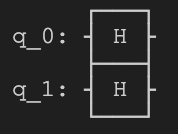
\includegraphics[width=0.25\linewidth]{circuit_superposition.png}
      \caption{Visualisierung des Schaltkreises (Superposition)}
      \label{fig:enter-label}
\end{figure}

\paragraph*{Visualisierung der Messergebnisse}
\mbox{}

Nach Ausführung des Algorithmus auf einem Quantensimulator – konkret dem QASM-Simulator von Qiskit – erfolgt die Analyse der Ergebnisse durch grafische Darstellung der Messausgänge.  Dabei wird die Methode \texttt{plot\_histogram()} verwendet, die ein Histogramm der gemessenen Zustände erzeugt.  Die Höhe der jeweiligen Balken repräsentiert die Häufigkeit (bzw. Wahrscheinlichkeit) eines bestimmten Bitmusters, das bei der Messung beobachtet wurde. 

Im Idealfall – das heißt, bei korrekter Funktionsweise des Orakels und des Grover-Operators – zeigt das Histogramm einen klar dominanten Peak beim Zielzustand.  Die Wahrscheinlichkeiten für alle anderen Zustände bleiben deutlich geringer.  Der gesuchte Zustand hebt sich somit durch quantenmechanische Verstärkung deutlich ab.  Der entsprechende Code zur Ergebnisvisualisierung lautet: 
\begin{verbatim}
plot_histogram(counts)
plt.show()
plot_histogram(counts)
plt.show()
\end{verbatim}

\begin{figure}
    \centering
    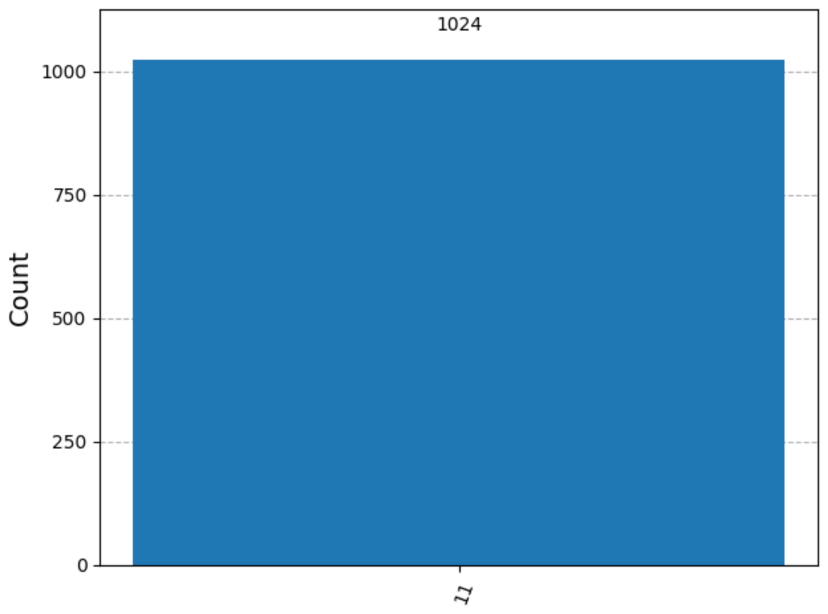
\includegraphics[width=0.75\linewidth]{Visualisierung der Messergebnisse.png}
    \caption{Visualisierung der Messergebnisse}
    \label{fig:enter-label}
\end{figure}

Die Kombination aus Schaltkreisvisualisierung und Ergebnisdarstellung bietet einen idealen Zugang zum Verständnis von Grovers Algorithmus.  Sie macht die Wirkung der einzelnen quantenlogischen Schritte nachvollziehbar und veranschaulicht das Prinzip der amplitudenbasierten Suche auf anschauliche Weise.  Solche Visualisierungen sind nicht nur didaktisch wertvoll, sondern auch essenziell für die Entwicklung und Analyse komplexerer Quantenalgorithmen in der Praxis. 

\clearpage % Fügt einen Seitenumbruch ein, um den nächsten Abschnitt auf einer neuen Seite zu beginnen

\subsubsection{Tests und Debugging-Hilfsmittel (z.\,B. Histogramme, Counts)}


\paragraph*{Tests und Debugging-Hilfsmittel}
\mbox{}

Bei der Entwicklung von Quantenalgorithmen spielt die systematische Überprüfung des Codes eine entscheidende Rolle, insbesondere im experimentellen Rahmen mit Frameworks wie Qiskit. Quantenprogramme sind nicht nur aufgrund ihrer Komplexität fehleranfällig, sondern verhalten sich auch häufig nicht intuitiv, da viele Zustände nicht direkt beobachtbar sind. Deshalb ist es essenziell, gezielt mit Tests, Zwischenergebnissen und Visualisierungen zu arbeiten, um Fehler zu erkennen und zu beheben.

\paragraph*{Schrittweise Entwicklung und Visualisierung}
\mbox{}

Im vorliegenden Notebook wurde der Grover-Algorithmus schrittweise aufgebaut, was eine erste Form des \enquote{Testens durch Design} darstellt. So wurden zunächst einzelne Operatoren und Zustände erzeugt, bevor sie in die Gesamtschaltung integriert wurden. Ein typisches Beispiel findet sich im Abschnitt zur 2-Qubit-Version:
\begin{verbatim}
def diffusion(circuit):
    circuit.h([0, 1])
    circuit.x([0, 1])
    circuit.h(1)
    circuit.cx(0, 1)
    circuit.h(1)
    circuit.x([0, 1])
    circuit.h([0, 1])
# Grover Circuit
grover_circ = QuantumCircuit(2)
grover_circ.h([0, 1])         # Superposition
oracle(grover_circ)           # Oracle anwenden
diffusion(grover_circ)        # Verstärkung
grover_circ.measure_all()
def diffusion(circuit):
    circuit.h([0, 1])
    circuit.x([0, 1])
    circuit.h(1)
    circuit.cx(0, 1)
    circuit.h(1)
    circuit.x([0, 1])
    circuit.h([0, 1])
# Grover Circuit
grover_circ = QuantumCircuit(2)
grover_circ.h([0, 1])         # Superposition
oracle(grover_circ)           # Oracle anwenden
diffusion(grover_circ)        # Verstärkung
grover_circ.measure_all()
\end{verbatim}
Durch das schrittweise Ergänzen der Gates kann bereits in frühen Phasen kontrolliert werden, ob jede Transformation wie gewünscht wirkt. Dies entspricht einem iterativen Debugging-Verfahren.

\paragraph*{Visualisierung als Debugging-Werkzeug}
\mbox{}

Wie im vorherigen Kapitel gezeigt, wird mit \texttt{draw()} der Schaltkreis visualisiert. Dies erfüllt nicht nur dokumentarische, sondern auch diagnostische Zwecke. Es kann dadurch überprüft werden, ob etwa das Oracle korrekt umgesetzt oder die Anzahl der Grover-Iterationen richtig gewählt wurde.
\subparagraph*{Beispiel:}
\begin{verbatim}
circuit.draw()
circuit.draw()
\end{verbatim}
Fehlende oder falsch platzierte Gates werden so unmittelbar sichtbar. Besonders hilfreich ist dies bei komplexeren Operatorfolgen wie in der 3-Qubit-Version.

\paragraph*{Ergebnisanalyse durch Histogramme}
\mbox{}

Ein sehr effektives Mittel zur Fehlererkennung ist die statistische Analyse der Ausgaben. Die mit \texttt{plot\_histogram()} erzeugten Verteilungen lassen Rückschlüsse auf das Verhalten des Algorithmus zu:
\begin{verbatim}
plot_histogram(result.get_counts())
plot_histogram(result.get_counts())
\end{verbatim}
Tritt der erwartete Peak beim Zielzustand nicht auf, kann dies auf einen Fehler im Oracle, in der Grover-Iteration oder in der Initialisierung hinweisen. Wurde beispielsweise ein falsches CZ-Gatter verwendet oder versehentlich eine falsche Qubit-Reihenfolge angesprochen, so verteilt sich die Wahrscheinlichkeitsmasse ungleichmäßig oder falsch.

\paragraph*{Fazit}
\mbox{}

Die Arbeit mit Quantenalgorithmen erfordert sowohl eine sorgfältige Teststrategie, klassische Softwareentwicklung aber auch eine strukturiertere Herangehensweise. Im Notebook werden bereits einfache Mittel wie Visualisierung, gezielte Zwischenschritte und Histogrammanalyse genutzt und sind eine große Hilfe beim Debugging. Für komplexere Algorithmen empfiehlt sich darüber hinaus der gezielte Einsatz von Statevector-Simulationen, Barrieren zur Strukturierung und die Ausgabe von Zwischenzuständen.

\subsection{Fazit und Ausblick}
\begin{itemize}
    \item Zusammenfassung der Entwicklungsschritte
    \item Stärken und Schwächen aktueller Toolchains
    \item Ausblick: Hybrid-Ansätze, komplexere Anwendungsfälle, Integration in klassische Softwarelandschaften
\end{itemize}

\printbibliography
